%----------------------------------------------------------------------------------------
%    PACKAGES AND THEMES
%----------------------------------------------------------------------------------------

\documentclass[aspectratio=169,xcolor=dvipsnames]{beamer}
%\usepackage{siunitx}
\usetheme{SimplePlus}
\input{macros}

\usepackage{tikz}
\usepackage{hyperref}
\usepackage{amsmath,amssymb,mathpartir,iris}

\usepackage{graphicx} % Allows including images
\usepackage{booktabs} % Allows the use of \toprule, \midrule and \bottomrule in tables
\usepackage{xcolor}
\usepackage{listings}
\newcommand{\assert}[1]{\{#1\}}
\usepackage[skins,theorems]{tcolorbox}
\tcbset{highlight math style={enhanced,
  colframe=red,colback=white,arc=0pt,boxrule=1pt}}
  
\usetikzlibrary{automata}
  \usetikzlibrary{
                shapes.multipart
                }
\usetikzlibrary{arrows,positioning,calc,backgrounds,positioning,fit,shapes,snakes,quotes,graphs}
% Thanks to Alex Kocurek's "A Quick TikZ Guide for Modal Logicians"
% http://www.actual.world/resources/tex/doc/TikZ.pdf
\tikzset{
modal/.style={>=stealth',shorten >=1pt,shorten <=1pt,auto,node distance=2.0cm,
semithick},
world/.style={circle,draw,minimum size=1cm,fill=gray!15},
point/.style={circle,draw,inner sep=0.5mm,fill=black},
reflexive above/.style={->,loop,looseness=7,in=120,out=60},
reflexive below/.style={->,loop,looseness=7,in=240,out=300},
reflexive left/.style={->,loop,looseness=7,in=150,out=210},
reflexive right/.style={->,loop,looseness=7,in=30,out=330}
}
\tikzset{
modalw/.style={font=\tiny,>=stealth',shorten >=1pt,shorten <=1pt,auto,node distance=0.8cm,
semithick},
world/.style={circle,draw,minimum size=0.75cm,fill=gray!15},
point/.style={circle,draw,inner sep=0.5mm,fill=black},
reflexive above/.style={->,loop,looseness=7,in=120,out=60},
reflexive below/.style={->,loop,looseness=7,in=240,out=300},
reflexive left/.style={->,loop,looseness=7,in=150,out=210},
reflexive right/.style={->,loop,looseness=7,in=30,out=330}
}
 \tikzstyle{background}=[circle split,
                                                    fill=gray!10,
                                                    inner sep=0.0001cm,
                                                    rounded corners=5mm]
 \tikzstyle{backgrounddiamond}=[rectangle,
                                                    fill=gray!10,
                                                    inner sep=0.2cm,
                                                    rounded corners=5mm]

\tikzstyle{background1}=[rectangle,
                                                    fill=darkgray!30,
                                                    inner sep=0.2cm,
                                                    rounded corners=5mm]

\tikzstyle{background2}=[rectangle,
                                                    fill=gray!60,
                                                    inner sep=0.2cm,
                                                    rounded corners=5mm]



\definecolor{mGreen}{rgb}{0,0.6,0}
\definecolor{mGray}{rgb}{0.5,0.5,0.5}
\definecolor{mPurple}{rgb}{0.58,0,0.82}
\definecolor{backgroundColour}{rgb}{0.95,0.95,0.92}
\lstdefinestyle{CStyleNum}{
    backgroundcolor=\color{backgroundColour},   
    commentstyle=\color{mGreen},
    keywordstyle=\color{magenta},
    numberstyle=\tiny\color{mGray},
    stringstyle=\color{mPurple},
    basicstyle=\scriptsize,
    breakatwhitespace=false,         
    breaklines=true,                 
    captionpos=b,                    
    keepspaces=true,                 
   % numbers=left,                    
   % numbersep=5pt,                  
    showspaces=false,                
    showstringspaces=false,
    showtabs=false,                  
   % tabsize=2,
    language=C
}
%,
        \lstdefinestyle{CStyleNumEmph}{
    backgroundcolor=\color{backgroundColour},   
    commentstyle=\color{mGreen},
    keywordstyle=\color{magenta},
    numberstyle=\tiny\color{mGray},
    stringstyle=\color{mPurple},
    basicstyle=\scriptsize,
    breakatwhitespace=false,         
    breaklines=true,                 
    captionpos=b,                    
    keepspaces=true,                 
   % numbers=left,                    
   % numbersep=5pt,                  
    showspaces=false,                
    showstringspaces=false,
    showtabs=false,                  
   % tabsize=2,
    language=C,
    \lstset{emph={P2V, next_virt_addr, next_phys_addr},emphstyle=\textbf}
}
\lstdefinestyle{CStyle}{
    backgroundcolor=\color{backgroundColour},   
    commentstyle=\color{mGreen},
    keywordstyle=\color{magenta},
    numberstyle=\tiny\color{mGray},
    stringstyle=\color{mPurple},
    basicstyle=\scriptsize,
    breakatwhitespace=false,         
    breaklines=true,                 
    captionpos=b,                    
    keepspaces=true,                 
    numbers=left,                    
    numbersep=5pt,                  
    showspaces=false,                
    showstringspaces=false,
    showtabs=false,                  
    tabsize=2,
    language=C
}
\newcommand{\sumwalkabsent}{
  \ownGhost\gammaPred{\authfrag{\singletonMap{\texttt{entry+KERNBASE}}{(\textsf{qfrac}, \textsf{entry})}}}
}

\newcommand{\gammaPred}{\delta}
\newcommand{\gammaPreds}{\delta\textsf{s}}
\newcommand{\rtv}{\textsf{rtv}}
\newcommand{\qone}{\texttt{q1}}
\newcommand{\qtwo}{\texttt{q2}}
\newcommand{\qthree}{\texttt{q3}}
\newcommand{\qfour}{\texttt{q4}}

\newcommand{\sumwalkabs}[3]{
  \ownGhost\gammaPred{\authfrag{\singletonMap{#1}{(#2, #3)}}}
}

\newcommand{\sumapaces}[2]{
  \ownGhost\gammaPreds{\authfrag{\singletonMap{#1}{#2}}}
}
\newcommand{\ptableabswalk}[1]{\mathcal{A}\textsf{bsPTableWalk}(#1)}
\newcommand{\ptablestore}{\theta}
\newcommand{\ventry}{\texttt{entry + KERNBASE}}
\newcommand{\entry}{\texttt{entry}}
\newcommand{\qfraczero}{\textsf{qfrac}}
\newcommand{\true}{\textsf{true}}
\tikzstyle{boxedassert_border} = [sharp corners,line width=0.2pt]
\NewDocumentCommand \boxedassertpv {O{} m o}{%
	\tikz[baseline=(m.base)]{
		%	  \node[rectangle, draw,inner sep=0.8pt,anchor=base,#1] (m) {${#2}\mathstrut$};
		\node[rectangle,inner sep=1.5pt,outer sep=0.2pt,anchor=base] (m) {${\,#2\,}\mathstrut$};
		\draw[#1,boxedassert_border] ($(m.south west)$) rectangle ($(m.north east)$);
	}\IfNoValueF{#3}{^{\,#3}}%
}
\newcommand*{\knowInvpv}[2]{\boxedassertpv{#2}[#1]}
\newcommand*{\ownGhostpv}[2]{\boxedassertpv[dash dot]{#2}[#1]}

\newcommand{\sumpv}[3]{
  \ownGhostpv\gammaPred{\authfrag{\singletonMap{#1}{(#2, #3)}}}
}
 % iris.sty lacks nice syntax for the ghost maps
  \newcommand{\ghostmaptoken}[3]{\ensuremath{#2\hookrightarrow^{#1}#3}}
  \newcommand{\fracghostmaptoken}[4]{\ensuremath{#2\hookrightarrow^{#1}_{#4}#3}}

\newcommand{\vale}{\textsf{val}}
\newcommand{\pvmapping}[1]{\mathcal{A}\textsf{PVMappings}(#1)}


\newcommand{\fpaddr}{\texttt{fpaddr}}
\newcommand{\specline}[1]{{\color{blue}\left\{#1\right\}}}
\newcommand{\sumapacesfull}[2]{
  \ownGhost\gammaPreds{\authfull{\singletonMap{#1}{#2}}}
}


\newcommand{\makepart}[1]{ % For convenience
\part{#1} \frame{\partpage}
%\section{Section} \begin{frame} Section \end{frame}
%\subsection{Subsection} \begin{frame} Subsection \end{frame}
%\subsection{Subsection} \begin{frame} Subsection \end{frame}
%\section{Section} \begin{frame} Section \end{frame}
}

%----------------------------------------------------------------------------------------
%    TITLE PAGE
%----------------------------------------------------------------------------------------

\title{Research Overview}
\subtitle{}

\author{Ismail Kuru}

\institute
{
    Department of Computer Science \\
    Drexel University % Your institution for the title page
}
\date{\today} % Date, can be changed to a custom date

%----------------------------------------------------------------------------------------
%    PRESENTATION SLIDES
%----------------------------------------------------------------------------------------

\begin{document}

\begin{frame}
    % Print the title page as the first slide
    \titlepage
\end{frame}

\begin{frame}{Overview}
\begin{itemize}
    \item Part I: Foundations for Location Virtualization
    \item Part II: Foundations for Specification Evolution
    \item Part III: Semantic Type Assertions for Deferred Memory-Reclamation Schemes
\end{itemize}

%\tableofcontents[part=1]

\end{frame}
%\begin{frame}{Overview}

%\tableofcontents[part=2]
  %  
%\end{frame}
\makepart{Modal Understanding of Location Virtualization}

%------------------------------------------------

%------------------------------------------------
\section{Definitions}
%------------------------

\begin{frame}[fragile]{The Essentials in Systems Programming}
\begin{lstlisting}[style=CStyle,mathescape]
    $\underbrace{\mathsf{pointer} \; \mathsf{va}}_{\mathsf{a\; virtual \;reference}}$ := $\overbrace{\mathsf{malloc\;(size)}}^{\mathsf{a \;supposedly \;allocated \;physical \;resource}}$
\end{lstlisting}
\end{frame}

\begin{frame}{Memory Location Virtualization}
   \begin{figure}
       \centering
   \tikzset{every picture/.style={line width=0.75pt}} %set default line width to 0.75pt        

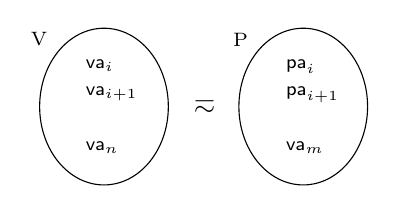
\begin{tikzpicture}[x=0.75pt,y=0.75pt,yscale=-0.5,xscale=0.5]
%uncomment if require: \path (0,176); %set diagram left start at 0, and has height of 176

%Shape: Ellipse [id:dp3089668103197505] 
\draw   (24,87.5) .. controls (24,45.8) and (51.76,12) .. (86,12) .. controls (120.24,12) and (148,45.8) .. (148,87.5) .. controls (148,129.2) and (120.24,163) .. (86,163) .. controls (51.76,163) and (24,129.2) .. (24,87.5) -- cycle ;
%Shape: Ellipse [id:dp3055465022453865] 
\draw   (216,87.5) .. controls (216,45.8) and (243.76,12) .. (278,12) .. controls (312.24,12) and (340,45.8) .. (340,87.5) .. controls (340,129.2) and (312.24,163) .. (278,163) .. controls (243.76,163) and (216,129.2) .. (216,87.5) -- cycle ;

% Text Node
\draw (13,13) node [anchor=north west][inner sep=0.75pt]   [align=left] {\scriptsize V};
% Text Node
\draw (208,14) node [anchor=north west][inner sep=0.75pt]   [align=left] {\scriptsize P};
% Text Node
\draw (170,79.4) node [anchor=north west][inner sep=0.75pt]    {$\eqsim $};
% Text Node
\draw (66,40) node [anchor=north west][inner sep=0.75pt]   [align=left] {\scriptsize $\mathsf{va}_i$};
% Text Node
\draw (66,66) node [anchor=north west][inner sep=0.75pt]   [align=left] {\scriptsize $\mathsf{va}_{i+1}$};
% Text Node
\draw (66,119) node [anchor=north west][inner sep=0.75pt]   [align=left] {\scriptsize $\mathsf{va}_n$};
% Text Node
\draw (259,40) node [anchor=north west][inner sep=0.75pt]   [align=left] {\scriptsize $\mathsf{pa}_i$};
% Text Node
\draw (259,66) node [anchor=north west][inner sep=0.75pt]   [align=left] {\scriptsize $\mathsf{pa}_{i+1}$};
% Text Node
\draw (259,119) node [anchor=north west][inner sep=0.75pt]   [align=left] {\scriptsize $\mathsf{va}_m$};


\end{tikzpicture}
       \caption{Virtualization: The Deception of Abundance}
       \label{fig:enter-label}
   \end{figure}
\end{frame}

%---------------------------------------------------
\begin{frame}[fragile]{Memory Location Virtualization: Abstraction}

  \begin{columns}[c] % The "c" option specifies centered vertical alignment while the "t" option is used for top vertical alignment

        \column{.45\textwidth} % Left column and width
        \textbf{An Address Space with Logical Name} $\gamma$
        \begin{figure}
    \centering
\tikzset{every picture/.style={line width=0.75pt}} %set default line width to 0.75pt        

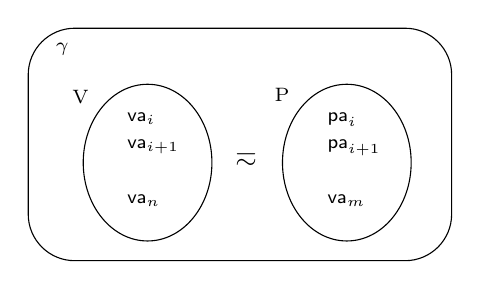
\begin{tikzpicture}[x=0.75pt,y=0.75pt,yscale=-0.5,xscale=0.5]
%uncomment if require: \path (0,250); %set diagram left start at 0, and has height of 250

%Shape: Ellipse [id:dp7871360559446556] 
\draw   (91,137.5) .. controls (91,95.8) and (118.76,62) .. (153,62) .. controls (187.24,62) and (215,95.8) .. (215,137.5) .. controls (215,179.2) and (187.24,213) .. (153,213) .. controls (118.76,213) and (91,179.2) .. (91,137.5) -- cycle ;
%Shape: Ellipse [id:dp9295032901075098] 
\draw   (283,137.5) .. controls (283,95.8) and (310.76,62) .. (345,62) .. controls (379.24,62) and (407,95.8) .. (407,137.5) .. controls (407,179.2) and (379.24,213) .. (345,213) .. controls (310.76,213) and (283,179.2) .. (283,137.5) -- cycle ;
%Rounded Rect [id:dp2598148010919421] 
\draw   (38,52.8) .. controls (38,28.06) and (58.06,8) .. (82.8,8) -- (401.2,8) .. controls (425.94,8) and (446,28.06) .. (446,52.8) -- (446,187.2) .. controls (446,211.94) and (425.94,232) .. (401.2,232) -- (82.8,232) .. controls (58.06,232) and (38,211.94) .. (38,187.2) -- cycle ;

% Text Node
\draw (78,65) node [anchor=north west][inner sep=0.75pt]   [align=left] {\scriptsize V};
% Text Node
\draw (273,63) node [anchor=north west][inner sep=0.75pt]   [align=left] {\scriptsize P};
% Text Node
\draw (235,126) node [anchor=north west][inner sep=0.75pt]    {$\eqsim $};
% Text Node
\draw (131,87) node [anchor=north west][inner sep=0.75pt]   [align=left] {\scriptsize $\mathsf{va}_i$};
% Text Node
\draw (131,113) node [anchor=north west][inner sep=0.75pt]   [align=left] {\scriptsize $\mathsf{va}_{i+1}$};
% Text Node
\draw (131,166) node [anchor=north west][inner sep=0.75pt]   [align=left] {\scriptsize $\mathsf{va}_n$};
% Text Node
\draw (324,87) node [anchor=north west][inner sep=0.75pt]   [align=left] {\scriptsize $\mathsf{pa}_i$};
% Text Node
\draw (324,113) node [anchor=north west][inner sep=0.75pt]   [align=left] {\scriptsize $\mathsf{pa}_{i+1}$};
% Text Node
\draw (324,166) node [anchor=north west][inner sep=0.75pt]   [align=left] {\scriptsize $\mathsf{va}_m$};
% Text Node
\draw (62,20) node [anchor=north west][inner sep=0.75pt]   [align=left] {\scriptsize $ \gamma $};


\end{tikzpicture}
   % In this slide, some important text will be \alert{highlighted} because it's important. Please, don't abuse it.

   % \begin{block}{Block}
   %     Sample text
   % \end{block}

%    \begin{alertblock}{Alertblock}
 %       Sample text in red box
 %   \end{alertblock}

  %  \begin{examples}
  %      Sample text in green box. The title of the block is ``Examples".
  %  \end{examples}
      \caption{Address-Spaces: Named Containers for Virtual Memory Mappings}
    \label{fig:enter-label}
\end{figure}

        \column{.45\textwidth} 
        \begin{columns}[c]
            \column{.55\textwidth}
            \textbf{A Program Named} $\gamma_n$
            \begin{lstlisting}[style=CStyleNum,mathescape]
    pointer va :=
     malloc(size)
\end{lstlisting}
            \column{.55\textwidth}
            \textbf{A Program Named} $\gamma_m$
            \begin{lstlisting}[style=CStyleNum,mathescape]
    pointer va := 
     malloc(size)
\end{lstlisting}
        \end{columns}
        \begin{itemize}
      \item  A program is abstracted as a \emph{named address-space}
      \item A container of \emph{virtual-to-physical} memory resource mappings
\end{itemize}
    \end{columns}
\end{frame}

%------------------------------------------------

%------------------------------------------------

\begin{frame}{Page Tables}
  

\begin{figure}
    \centering



\tikzset{every picture/.style={line width=0.75pt}} %set default line width to 0.75pt        

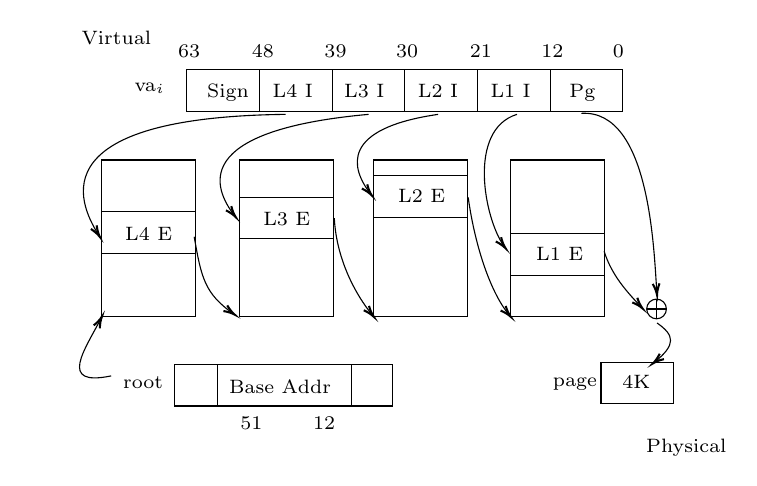
\begin{tikzpicture}[x=0.75pt,y=0.75pt,yscale=-0.5,xscale=0.5]
%uncomment if require: \path (0,444); %set diagram left start at 0, and has height of 444

%Shape: Rectangle [id:dp9406932326447903] 
\draw   (33,141) -- (123,141) -- (123,292) -- (33,292) -- cycle ;
%Shape: Rectangle [id:dp7682116051394419] 
\draw   (166,141) -- (256,141) -- (256,292) -- (166,292) -- cycle ;
%Shape: Rectangle [id:dp07376733516930423] 
\draw   (295,141) -- (385,141) -- (385,292) -- (295,292) -- cycle ;
%Shape: Rectangle [id:dp7106629147891306] 
\draw   (427,141) -- (517,141) -- (517,292) -- (427,292) -- cycle ;
%Shape: Rectangle [id:dp1342906826203598] 
\draw   (115,54) -- (185,54) -- (185,94) -- (115,94) -- cycle ;
%Shape: Rectangle [id:dp08072439007207399] 
\draw   (185,54) -- (255,54) -- (255,94) -- (185,94) -- cycle ;
%Shape: Rectangle [id:dp8282933603833216] 
\draw   (255,54) -- (325,54) -- (325,94) -- (255,94) -- cycle ;
%Shape: Rectangle [id:dp8416255090865326] 
\draw   (325,54) -- (395,54) -- (395,94) -- (325,94) -- cycle ;
%Shape: Rectangle [id:dp22911958218529804] 
\draw   (395,54) -- (465,54) -- (465,94) -- (395,94) -- cycle ;
%Shape: Rectangle [id:dp33732955213990756] 
\draw   (465,54) -- (535,54) -- (535,94) -- (465,94) -- cycle ;
%Curve Lines [id:da6688730321284677] 
\draw    (210,97) .. controls (-37.94,99.94) and (15.69,190.28) .. (30.17,213.65) ;
\draw [shift={(31,215)}, rotate = 238.24] [color={rgb, 255:red, 0; green, 0; blue, 0 }  ][line width=0.75]    (10.93,-3.29) .. controls (6.95,-1.4) and (3.31,-0.3) .. (0,0) .. controls (3.31,0.3) and (6.95,1.4) .. (10.93,3.29)   ;
%Shape: Rectangle [id:dp6044747978986409] 
\draw   (33,191) -- (123,191) -- (123,231) -- (33,231) -- cycle ;
%Curve Lines [id:da8867562998134584] 
\draw    (290,97) .. controls (116.54,112.68) and (140.92,168.7) .. (160.79,194.46) ;
\draw [shift={(162,196)}, rotate = 231.34] [color={rgb, 255:red, 0; green, 0; blue, 0 }  ][line width=0.75]    (10.93,-3.29) .. controls (6.95,-1.4) and (3.31,-0.3) .. (0,0) .. controls (3.31,0.3) and (6.95,1.4) .. (10.93,3.29)   ;
%Shape: Rectangle [id:dp8861153167245819] 
\draw   (166,177) -- (256,177) -- (256,217) -- (166,217) -- cycle ;
%Shape: Rectangle [id:dp05979844200848894] 
\draw   (295,156) -- (385,156) -- (385,196) -- (295,196) -- cycle ;
%Shape: Rectangle [id:dp17403733244247843] 
\draw   (427,212) -- (517,212) -- (517,252) -- (427,252) -- cycle ;
%Curve Lines [id:da20581124900573955] 
\draw    (357,97) .. controls (262.92,110.72) and (272.56,148.45) .. (291.81,173.48) ;
\draw [shift={(293,175)}, rotate = 231.34] [color={rgb, 255:red, 0; green, 0; blue, 0 }  ][line width=0.75]    (10.93,-3.29) .. controls (6.95,-1.4) and (3.31,-0.3) .. (0,0) .. controls (3.31,0.3) and (6.95,1.4) .. (10.93,3.29)   ;
%Curve Lines [id:da07589611603635316] 
\draw    (433,97) .. controls (384.98,111.7) and (401.31,197.47) .. (420.8,224.42) ;
\draw [shift={(422,226)}, rotate = 231.34] [color={rgb, 255:red, 0; green, 0; blue, 0 }  ][line width=0.75]    (10.93,-3.29) .. controls (6.95,-1.4) and (3.31,-0.3) .. (0,0) .. controls (3.31,0.3) and (6.95,1.4) .. (10.93,3.29)   ;
%Curve Lines [id:da6852167546673456] 
\draw    (495,96) .. controls (561.98,92.06) and (564.93,230.74) .. (567.87,269.31) ;
\draw [shift={(568,271)}, rotate = 265.24] [color={rgb, 255:red, 0; green, 0; blue, 0 }  ][line width=0.75]    (10.93,-3.29) .. controls (6.95,-1.4) and (3.31,-0.3) .. (0,0) .. controls (3.31,0.3) and (6.95,1.4) .. (10.93,3.29)   ;
%Curve Lines [id:da017521077423665377] 
\draw    (42,349) .. controls (-10.21,359.84) and (17.15,323.13) .. (32.32,293.36) ;
\draw [shift={(33,292)}, rotate = 116.57] [color={rgb, 255:red, 0; green, 0; blue, 0 }  ][line width=0.75]    (10.93,-3.29) .. controls (6.95,-1.4) and (3.31,-0.3) .. (0,0) .. controls (3.31,0.3) and (6.95,1.4) .. (10.93,3.29)   ;
%Curve Lines [id:da6750042432035159] 
\draw    (122,215) .. controls (128.9,254.4) and (131.91,269.54) .. (159.71,289.1) ;
\draw [shift={(161,290)}, rotate = 214.59] [color={rgb, 255:red, 0; green, 0; blue, 0 }  ][line width=0.75]    (10.93,-3.29) .. controls (6.95,-1.4) and (3.31,-0.3) .. (0,0) .. controls (3.31,0.3) and (6.95,1.4) .. (10.93,3.29)   ;
%Curve Lines [id:da14788158682113428] 
\draw    (257,197) .. controls (258.95,236) and (277.06,270.25) .. (293.72,290.47) ;
\draw [shift={(295,292)}, rotate = 229.64] [color={rgb, 255:red, 0; green, 0; blue, 0 }  ][line width=0.75]    (10.93,-3.29) .. controls (6.95,-1.4) and (3.31,-0.3) .. (0,0) .. controls (3.31,0.3) and (6.95,1.4) .. (10.93,3.29)   ;
%Curve Lines [id:da3297977595767969] 
\draw    (386,177) .. controls (392.86,226) and (408.36,270.2) .. (425.92,290.77) ;
\draw [shift={(427,292)}, rotate = 228.01] [color={rgb, 255:red, 0; green, 0; blue, 0 }  ][line width=0.75]    (10.93,-3.29) .. controls (6.95,-1.4) and (3.31,-0.3) .. (0,0) .. controls (3.31,0.3) and (6.95,1.4) .. (10.93,3.29)   ;
%Curve Lines [id:da7710391961792686] 
\draw    (517,229) .. controls (524.76,253.25) and (540.05,269.03) .. (552.82,282.73) ;
\draw [shift={(554,284)}, rotate = 227.12] [color={rgb, 255:red, 0; green, 0; blue, 0 }  ][line width=0.75]    (10.93,-3.29) .. controls (6.95,-1.4) and (3.31,-0.3) .. (0,0) .. controls (3.31,0.3) and (6.95,1.4) .. (10.93,3.29)   ;
%Shape: Rectangle [id:dp1535611125971872] 
\draw   (514,336) -- (584,336) -- (584,376) -- (514,376) -- cycle ;
%Shape: Rectangle [id:dp05427947476226991] 
\draw   (103,338) -- (144.5,338) -- (144.5,378) -- (103,378) -- cycle ;
%Shape: Rectangle [id:dp10511138743752002] 
\draw   (144.5,338) -- (273.5,338) -- (273.5,378) -- (144.5,378) -- cycle ;
%Shape: Rectangle [id:dp8917680919534263] 
\draw   (273.5,338) -- (313,338) -- (313,378) -- (273.5,378) -- cycle ;
\draw   (558,284.5) .. controls (558,279.25) and (562.25,275) .. (567.5,275) .. controls (572.75,275) and (577,279.25) .. (577,284.5) .. controls (577,289.75) and (572.75,294) .. (567.5,294) .. controls (562.25,294) and (558,289.75) .. (558,284.5) -- cycle ; \draw   (558,284.5) -- (577,284.5) ; \draw   (567.5,275) -- (567.5,294) ;
%Curve Lines [id:da9312068388962929] 
\draw    (568,298) .. controls (584.66,309.76) and (586.91,318.64) .. (565.35,335.93) ;
\draw [shift={(564,337)}, rotate = 321.95] [color={rgb, 255:red, 0; green, 0; blue, 0 }  ][line width=0.75]    (10.93,-3.29) .. controls (6.95,-1.4) and (3.31,-0.3) .. (0,0) .. controls (3.31,0.3) and (6.95,1.4) .. (10.93,3.29)   ;

% Text Node
\draw (11,14) node [anchor=north west][inner sep=0.75pt]   [align=left] {{\scriptsize Virtual}};
% Text Node
\draw (555,407) node [anchor=north west][inner sep=0.75pt]   [align=left] {{\scriptsize Physical}};
% Text Node
\draw (104,28) node [anchor=north west][inner sep=0.75pt]   [align=left] {{\scriptsize 63}};
% Text Node
\draw (175,28) node [anchor=north west][inner sep=0.75pt]   [align=left] {{\scriptsize 48}};
% Text Node
\draw (245,28) node [anchor=north west][inner sep=0.75pt]   [align=left] {{\scriptsize 39}};
% Text Node
\draw (314,28) node [anchor=north west][inner sep=0.75pt]   [align=left] {{\scriptsize 30}};
% Text Node
\draw (385,28) node [anchor=north west][inner sep=0.75pt]   [align=left] {{\scriptsize 21}};
% Text Node
\draw (454,28) node [anchor=north west][inner sep=0.75pt]   [align=left] {{\scriptsize 12}};
% Text Node
\draw (523,28) node [anchor=north west][inner sep=0.75pt]   [align=left] {{\scriptsize 0}};
% Text Node
\draw (132,65) node [anchor=north west][inner sep=0.75pt]   [align=left] {{\scriptsize Sign}};
% Text Node
\draw (195,65) node [anchor=north west][inner sep=0.75pt]   [align=left] {{\scriptsize L4 I}};
% Text Node
\draw (264,65) node [anchor=north west][inner sep=0.75pt]   [align=left] {{\scriptsize L3 I}};
% Text Node
\draw (335,65) node [anchor=north west][inner sep=0.75pt]   [align=left] {{\scriptsize L2 I}};
% Text Node
\draw (405,65) node [anchor=north west][inner sep=0.75pt]   [align=left] {{\scriptsize L1 I}};
% Text Node
\draw (481,65) node [anchor=north west][inner sep=0.75pt]   [align=left] {{\scriptsize Pg}};
% Text Node
\draw (62,64) node [anchor=north west][inner sep=0.75pt]   [align=left] {{\scriptsize va$_i$}};
% Text Node
\draw (53,203) node [anchor=north west][inner sep=0.75pt]   [align=left] {{\scriptsize L4 E}};
% Text Node
\draw (186,189) node [anchor=north west][inner sep=0.75pt]   [align=left] {{\scriptsize L3 E}};
% Text Node
\draw (316,167) node [anchor=north west][inner sep=0.75pt]   [align=left] {{\scriptsize L2 E}};
% Text Node
\draw (449,223) node [anchor=north west][inner sep=0.75pt]   [align=left] {{\scriptsize L1 E}};
% Text Node
\draw (51,347) node [anchor=north west][inner sep=0.75pt]   [align=left] {{\scriptsize root}};
% Text Node
\draw (465,349) node [anchor=north west][inner sep=0.75pt]   [align=left] {{\scriptsize page}};
% Text Node
\draw (532,346) node [anchor=north west][inner sep=0.75pt]   [align=left] {{\scriptsize 4K}};
% Text Node
\draw (164,386) node [anchor=north west][inner sep=0.75pt]   [align=left] {{\scriptsize 51}};
% Text Node
\draw (234,386) node [anchor=north west][inner sep=0.75pt]   [align=left] {{\scriptsize 12}};
% Text Node
\draw (153,350) node [anchor=north west][inner sep=0.75pt]   [align=left] {{\scriptsize Base Addr}};


\end{tikzpicture}
    \caption{Page-Tables (\textbf{PT}): Data Structures for Address-Translation}
    \label{fig:enter-label}
\end{figure}
\end{frame}

%------------------------------------------------
\begin{frame}{A Complete Picture of Address-Space Abstraction}
\begin{columns}[c]
\column{.35\textwidth}    
\begin{figure}
    \centering
    


\tikzset{every picture/.style={line width=0.75pt}} %set default line width to 0.75pt        

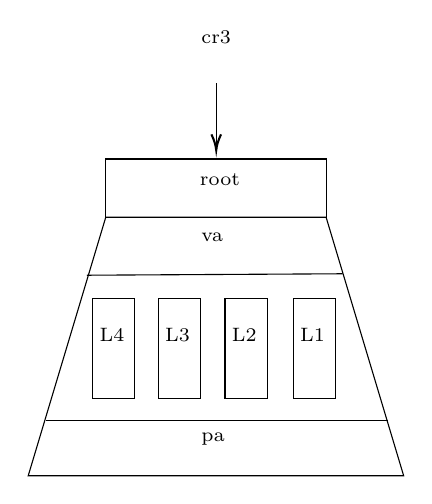
\begin{tikzpicture}[x=0.75pt,y=0.75pt,yscale=-0.7,xscale=0.7]
%uncomment if require: \path (0,361); %set diagram left start at 0, and has height of 361

%Straight Lines [id:da9421316390034546] 
\draw    (150,49) -- (150,93) ;
\draw [shift={(150,95)}, rotate = 270] [color={rgb, 255:red, 0; green, 0; blue, 0 }  ][line width=0.75]    (10.93,-3.29) .. controls (6.95,-1.4) and (3.31,-0.3) .. (0,0) .. controls (3.31,0.3) and (6.95,1.4) .. (10.93,3.29)   ;
%Shape: Trapezoid [id:dp42196090147818355] 
\draw   (20.6,319) -- (74,141) -- (225.6,141) -- (279,319) -- cycle ;
%Shape: Rectangle [id:dp05833798878152763] 
\draw   (74,101) -- (226,101) -- (226,141) -- (74,141) -- cycle ;
%Straight Lines [id:da5475026726551153] 
\draw    (61,181) -- (237,180) ;
%Straight Lines [id:da567347542499933] 
\draw    (33,281) -- (268,281) ;
%Shape: Rectangle [id:dp8593208287745469] 
\draw   (65,197) -- (94,197) -- (94,266) -- (65,266) -- cycle ;
%Shape: Rectangle [id:dp07187149088731903] 
\draw   (110,197) -- (139,197) -- (139,266) -- (110,266) -- cycle ;
%Shape: Rectangle [id:dp13017365116217516] 
\draw   (156,197) -- (185,197) -- (185,266) -- (156,266) -- cycle ;
%Shape: Rectangle [id:dp8238066656621155] 
\draw   (203,197) -- (232,197) -- (232,266) -- (203,266) -- cycle ;

% Text Node
\draw (138,11) node [anchor=north west][inner sep=0.75pt]   [align=left] {{\scriptsize cr3}};
% Text Node
\draw (138,150) node [anchor=north west][inner sep=0.75pt]   [align=left] {{\scriptsize va}};
% Text Node
\draw (138,288) node [anchor=north west][inner sep=0.75pt]   [align=left] {{\scriptsize pa}};
% Text Node
\draw (68,216) node [anchor=north west][inner sep=0.75pt]   [align=left] {{\scriptsize L4}};
% Text Node
\draw (113,216) node [anchor=north west][inner sep=0.75pt]   [align=left] {{\scriptsize L3}};
% Text Node
\draw (159,216) node [anchor=north west][inner sep=0.75pt]   [align=left] {{\scriptsize L2}};
% Text Node
\draw (206,216) node [anchor=north west][inner sep=0.75pt]   [align=left] {{\scriptsize L1}};
% Text Node
\draw (137,109) node [anchor=north west][inner sep=0.75pt]   [align=left] {{\scriptsize root}};


\end{tikzpicture}
    \caption{Depicting an Address-Space with its Essential Aspects}
    \label{fig:enter-label}
\end{figure}
\column{.6\textwidth}
  \begin{block}{The Current View of Memory}
    The register $\mathsf{cr}_3$ points to the current view of the memory, i.e., the loaded address space in the memory \end{block}.
\end{columns}

\end{frame}

\section{Motivation}
\begin{frame}{Virtual Memory Management (\textbf{VMM})}
    \begin{block}{\textbf{VMM} as a General Resource Provider}
    "the virtual memory sub-system can be considered the core of a Solaris instance, and the implementation of Solaris virtual memory affects just about every other subsystem in the operating system" \cite{mcdougall2006solaris}
    \end{block}
\end{frame}

%------------------------------------------------
\subsection{Sharing}

%Sharing Physical Page Tables 
%1.------------------------------------------------
%Sharing Physical Page Tables
%2--------------------------------------------------

%13--------------------------------------------------------
%14----------------------------------------------------------
\begin{frame}[fragile]{Sharing Physical Page Tables}

\begin{columns}[c]
\column{.59\textwidth}    
    \begin{figure}
        \centering
\tikzset{every picture/.style={line width=0.75pt}} %set default line width to 0.75pt        
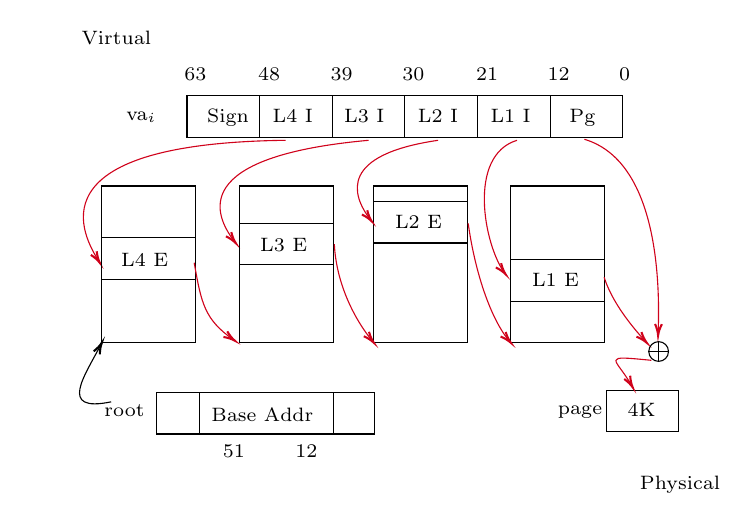
\begin{tikzpicture}[x=0.75pt,y=0.75pt,yscale=-0.5,xscale=0.5]
%uncomment if require: \path (0,471); %set diagram left start at 0, and has height of 471

%Shape: Rectangle [id:dp6797306099675045] 
\draw   (34,165) -- (124,165) -- (124,316) -- (34,316) -- cycle ;
%Shape: Rectangle [id:dp6192113478200691] 
\draw   (167,165) -- (257,165) -- (257,316) -- (167,316) -- cycle ;
%Shape: Rectangle [id:dp046479372017499854] 
\draw   (296,165) -- (386,165) -- (386,316) -- (296,316) -- cycle ;
%Shape: Rectangle [id:dp1806612887251846] 
\draw   (428,165) -- (518,165) -- (518,316) -- (428,316) -- cycle ;
%Shape: Rectangle [id:dp16201905390239735] 
\draw   (116,78) -- (186,78) -- (186,118) -- (116,118) -- cycle ;
%Shape: Rectangle [id:dp46359313115432044] 
\draw   (186,78) -- (256,78) -- (256,118) -- (186,118) -- cycle ;
%Shape: Rectangle [id:dp8986469180554777] 
\draw   (256,78) -- (326,78) -- (326,118) -- (256,118) -- cycle ;
%Shape: Rectangle [id:dp3960250568381902] 
\draw   (326,78) -- (396,78) -- (396,118) -- (326,118) -- cycle ;
%Shape: Rectangle [id:dp76786771788994] 
\draw   (396,78) -- (466,78) -- (466,118) -- (396,118) -- cycle ;
%Shape: Rectangle [id:dp9070245370995538] 
\draw   (466,78) -- (536,78) -- (536,118) -- (466,118) -- cycle ;
%Curve Lines [id:da6951218383977624] 
\draw [color={rgb, 255:red, 208; green, 2; blue, 27 }  ,draw opacity=1 ]   (211,121) .. controls (-36.94,123.94) and (16.69,214.28) .. (31.17,237.65) ;
\draw [shift={(32,239)}, rotate = 238.24] [color={rgb, 255:red, 208; green, 2; blue, 27 }  ,draw opacity=1 ][line width=0.75]    (10.93,-3.29) .. controls (6.95,-1.4) and (3.31,-0.3) .. (0,0) .. controls (3.31,0.3) and (6.95,1.4) .. (10.93,3.29)   ;
%Shape: Rectangle [id:dp48687197518810277] 
\draw   (34,215) -- (124,215) -- (124,255) -- (34,255) -- cycle ;
%Curve Lines [id:da7139570096435448] 
\draw [color={rgb, 255:red, 208; green, 2; blue, 27 }  ,draw opacity=1 ]   (291,121) .. controls (117.54,136.68) and (141.92,192.7) .. (161.79,218.46) ;
\draw [shift={(163,220)}, rotate = 231.34] [color={rgb, 255:red, 208; green, 2; blue, 27 }  ,draw opacity=1 ][line width=0.75]    (10.93,-3.29) .. controls (6.95,-1.4) and (3.31,-0.3) .. (0,0) .. controls (3.31,0.3) and (6.95,1.4) .. (10.93,3.29)   ;
%Shape: Rectangle [id:dp32338125663089956] 
\draw   (167,201) -- (257,201) -- (257,241) -- (167,241) -- cycle ;
%Shape: Rectangle [id:dp6104052627034173] 
\draw   (296,180) -- (386,180) -- (386,220) -- (296,220) -- cycle ;
%Shape: Rectangle [id:dp49476345634718477] 
\draw   (428,236) -- (518,236) -- (518,276) -- (428,276) -- cycle ;
%Curve Lines [id:da3926551025530285] 
\draw [color={rgb, 255:red, 208; green, 2; blue, 27 }  ,draw opacity=1 ]   (358,121) .. controls (263.92,134.72) and (273.56,172.45) .. (292.81,197.48) ;
\draw [shift={(294,199)}, rotate = 231.34] [color={rgb, 255:red, 208; green, 2; blue, 27 }  ,draw opacity=1 ][line width=0.75]    (10.93,-3.29) .. controls (6.95,-1.4) and (3.31,-0.3) .. (0,0) .. controls (3.31,0.3) and (6.95,1.4) .. (10.93,3.29)   ;
%Curve Lines [id:da38615138851194764] 
\draw [color={rgb, 255:red, 208; green, 2; blue, 27 }  ,draw opacity=1 ]   (434,121) .. controls (385.98,135.7) and (402.31,221.47) .. (421.8,248.42) ;
\draw [shift={(423,250)}, rotate = 231.34] [color={rgb, 255:red, 208; green, 2; blue, 27 }  ,draw opacity=1 ][line width=0.75]    (10.93,-3.29) .. controls (6.95,-1.4) and (3.31,-0.3) .. (0,0) .. controls (3.31,0.3) and (6.95,1.4) .. (10.93,3.29)   ;
%Curve Lines [id:da8796700124764012] 
\draw [color={rgb, 255:red, 208; green, 2; blue, 27 }  ,draw opacity=1 ]   (499,120) .. controls (574.46,142.54) and (571.17,273.61) .. (570.06,307.07) ;
\draw [shift={(570,309)}, rotate = 271.91] [color={rgb, 255:red, 208; green, 2; blue, 27 }  ,draw opacity=1 ][line width=0.75]    (10.93,-3.29) .. controls (6.95,-1.4) and (3.31,-0.3) .. (0,0) .. controls (3.31,0.3) and (6.95,1.4) .. (10.93,3.29)   ;
%Curve Lines [id:da26463336009584704] 
\draw    (43,373) .. controls (-9.21,383.84) and (18.15,347.13) .. (33.32,317.36) ;
\draw [shift={(34,316)}, rotate = 116.57] [color={rgb, 255:red, 0; green, 0; blue, 0 }  ][line width=0.75]    (10.93,-3.29) .. controls (6.95,-1.4) and (3.31,-0.3) .. (0,0) .. controls (3.31,0.3) and (6.95,1.4) .. (10.93,3.29)   ;
%Curve Lines [id:da18202057955172246] 
\draw [color={rgb, 255:red, 208; green, 2; blue, 27 }  ,draw opacity=1 ]   (123,239) .. controls (129.9,278.4) and (132.91,293.54) .. (160.71,313.1) ;
\draw [shift={(162,314)}, rotate = 214.59] [color={rgb, 255:red, 208; green, 2; blue, 27 }  ,draw opacity=1 ][line width=0.75]    (10.93,-3.29) .. controls (6.95,-1.4) and (3.31,-0.3) .. (0,0) .. controls (3.31,0.3) and (6.95,1.4) .. (10.93,3.29)   ;
%Curve Lines [id:da39925694981212034] 
\draw [color={rgb, 255:red, 208; green, 2; blue, 27 }  ,draw opacity=1 ]   (258,221) .. controls (259.95,260) and (278.06,294.25) .. (294.72,314.47) ;
\draw [shift={(296,316)}, rotate = 229.64] [color={rgb, 255:red, 208; green, 2; blue, 27 }  ,draw opacity=1 ][line width=0.75]    (10.93,-3.29) .. controls (6.95,-1.4) and (3.31,-0.3) .. (0,0) .. controls (3.31,0.3) and (6.95,1.4) .. (10.93,3.29)   ;
%Curve Lines [id:da0025982000064483923] 
\draw [color={rgb, 255:red, 208; green, 2; blue, 27 }  ,draw opacity=1 ]   (387,201) .. controls (393.86,250) and (409.36,294.2) .. (426.92,314.77) ;
\draw [shift={(428,316)}, rotate = 228.01] [color={rgb, 255:red, 208; green, 2; blue, 27 }  ,draw opacity=1 ][line width=0.75]    (10.93,-3.29) .. controls (6.95,-1.4) and (3.31,-0.3) .. (0,0) .. controls (3.31,0.3) and (6.95,1.4) .. (10.93,3.29)   ;
%Curve Lines [id:da4425456634879614] 
\draw [color={rgb, 255:red, 208; green, 2; blue, 27 }  ,draw opacity=1 ]   (518,253) .. controls (525.76,277.25) and (544.81,300.56) .. (557.81,314.71) ;
\draw [shift={(559,316)}, rotate = 227.12] [color={rgb, 255:red, 208; green, 2; blue, 27 }  ,draw opacity=1 ][line width=0.75]    (10.93,-3.29) .. controls (6.95,-1.4) and (3.31,-0.3) .. (0,0) .. controls (3.31,0.3) and (6.95,1.4) .. (10.93,3.29)   ;
%Shape: Rectangle [id:dp20590678105984384] 
\draw   (520,362) -- (590,362) -- (590,402) -- (520,402) -- cycle ;
%Shape: Rectangle [id:dp8145206670609288] 
\draw   (87,364) -- (128.5,364) -- (128.5,404) -- (87,404) -- cycle ;
%Shape: Rectangle [id:dp5322999267202655] 
\draw   (128.5,364) -- (257.5,364) -- (257.5,404) -- (128.5,404) -- cycle ;
%Shape: Rectangle [id:dp44035388924299834] 
\draw   (257.5,364) -- (297,364) -- (297,404) -- (257.5,404) -- cycle ;
\draw   (561,324.5) .. controls (561,319.25) and (565.25,315) .. (570.5,315) .. controls (575.75,315) and (580,319.25) .. (580,324.5) .. controls (580,329.75) and (575.75,334) .. (570.5,334) .. controls (565.25,334) and (561,329.75) .. (561,324.5) -- cycle ; \draw   (561,324.5) -- (580,324.5) ; \draw   (570.5,315) -- (570.5,334) ;
%Curve Lines [id:da7994290642535546] 
\draw [color={rgb, 255:red, 208; green, 2; blue, 27 }  ,draw opacity=1 ]   (563.5,333) .. controls (513.52,328.1) and (528.85,329.92) .. (544.54,357.29) ;
\draw [shift={(545.5,359)}, rotate = 241.11] [color={rgb, 255:red, 208; green, 2; blue, 27 }  ,draw opacity=1 ][line width=0.75]    (10.93,-3.29) .. controls (6.95,-1.4) and (3.31,-0.3) .. (0,0) .. controls (3.31,0.3) and (6.95,1.4) .. (10.93,3.29)   ;

% Text Node
\draw (12,13) node [anchor=north west][inner sep=0.75pt]   [align=left] {{\scriptsize Virtual}};
% Text Node
\draw (550,442) node [anchor=north west][inner sep=0.75pt]   [align=left] {{\scriptsize Physical}};
% Text Node
\draw (133,89) node [anchor=north west][inner sep=0.75pt]   [align=left] {{\scriptsize Sign}};
% Text Node
\draw (196,89) node [anchor=north west][inner sep=0.75pt]   [align=left] {{\scriptsize L4 I}};
% Text Node
\draw (265,89) node [anchor=north west][inner sep=0.75pt]   [align=left] {{\scriptsize L3 I}};
% Text Node
\draw (336,89) node [anchor=north west][inner sep=0.75pt]   [align=left] {{\scriptsize L2 I}};
% Text Node
\draw (406,89) node [anchor=north west][inner sep=0.75pt]   [align=left] {{\scriptsize L1 I}};
% Text Node
\draw (482,89) node [anchor=north west][inner sep=0.75pt]   [align=left] {{\scriptsize Pg}};
% Text Node
\draw (55,91) node [anchor=north west][inner sep=0.75pt]   [align=left] {{\scriptsize va$_i$}};
% Text Node
\draw (34,373) node [anchor=north west][inner sep=0.75pt]   [align=left] {{\scriptsize root}};
% Text Node
\draw (50,227) node [anchor=north west][inner sep=0.75pt]   [align=left] {{\scriptsize L4 E}};
% Text Node
\draw (184,213) node [anchor=north west][inner sep=0.75pt]   [align=left] {{\scriptsize L3 E}};
% Text Node
\draw (314,191) node [anchor=north west][inner sep=0.75pt]   [align=left] {{\scriptsize L2 E}};
% Text Node
\draw (446,247) node [anchor=north west][inner sep=0.75pt]   [align=left] {{\scriptsize L1 E}};
% Text Node
\draw (471,375) node [anchor=north west][inner sep=0.75pt]   [align=left] {{\scriptsize page}};
% Text Node
\draw (538,372) node [anchor=north west][inner sep=0.75pt]   [align=left] {{\scriptsize 4K}};
% Text Node
\draw (148,412) node [anchor=north west][inner sep=0.75pt]   [align=left] {{\scriptsize 51}};
% Text Node
\draw (218,412) node [anchor=north west][inner sep=0.75pt]   [align=left] {{\scriptsize 12}};
% Text Node
\draw (137,376) node [anchor=north west][inner sep=0.75pt]   [align=left] {{\scriptsize Base Addr}};
% Text Node
\draw (111,49) node [anchor=north west][inner sep=0.75pt]   [align=left] {{\scriptsize 63}};
% Text Node
\draw (182,49) node [anchor=north west][inner sep=0.75pt]   [align=left] {{\scriptsize 48}};
% Text Node
\draw (252,49) node [anchor=north west][inner sep=0.75pt]   [align=left] {{\scriptsize 39}};
% Text Node
\draw (321,49) node [anchor=north west][inner sep=0.75pt]   [align=left] {{\scriptsize 30}};
% Text Node
\draw (392,49) node [anchor=north west][inner sep=0.75pt]   [align=left] {{\scriptsize 21}};
% Text Node
\draw (461,49) node [anchor=north west][inner sep=0.75pt]   [align=left] {{\scriptsize 12}};
% Text Node
\draw (530,49) node [anchor=north west][inner sep=0.75pt]   [align=left] {{\scriptsize 0}};


\end{tikzpicture}
          \caption{Accessing to the Page Referenced by L1 Entry}
        \label{fig:enter-label}
    \end{figure}
    \column{.4\textwidth}
\begin{lstlisting}[style=CStyleNum, basicstyle=\tiny]
static pte_t *pte_nxt_table (pte_t *entry){
 pte_t *next;
 // If not already present, try to allocate
 if (!entry->present){
  if (!pte_alloc(&next)) {
   return NULL;
  }
  entry->pfn = PTE_PFN((uintptr_t) next);
  entry->present = 1;
  } else {
   uintptr_t next_phys_addr = PTE_PFN_TO_ADDR(entry->pfn);        
   uintptr_t next_virt_addr = (uintptr_t) P2V(next_phys_addr);
   next = (pte_t *) next_virt_addr;
  }
  return next;
}   
pte_t *walkpgdir(pte_t *l4, void *va){ 
 pte_t *l4_entry = &l4[L4I(va)];
 pte_t *l3 = pte_nxt_table(l4_entry);
 pte_t *l3_entry = &l3[L3I(va)];
 pte_t *l2 = pte_nxt_table(l3_entry);
 pte_t *l2_entry = &l2[L2I(va)];  
 pte_t *l1 = pte_nxt_table(l2_entry);
 pte_t *l1_entry = &l1[L1I(va)];  
 return l1_entry
}
\end{lstlisting}
\end{columns}
\end{frame}

%Soundness of Page Table Traversal
%--------------------------------------------
\begin{frame}{Breaking Soundness in Sharing}
\begin{columns}[c]
    \column{0.65\textwidth}
    \begin{figure}
        \centering
\tikzset{every picture/.style={line width=0.75pt}} %set default line width to 0.75pt        
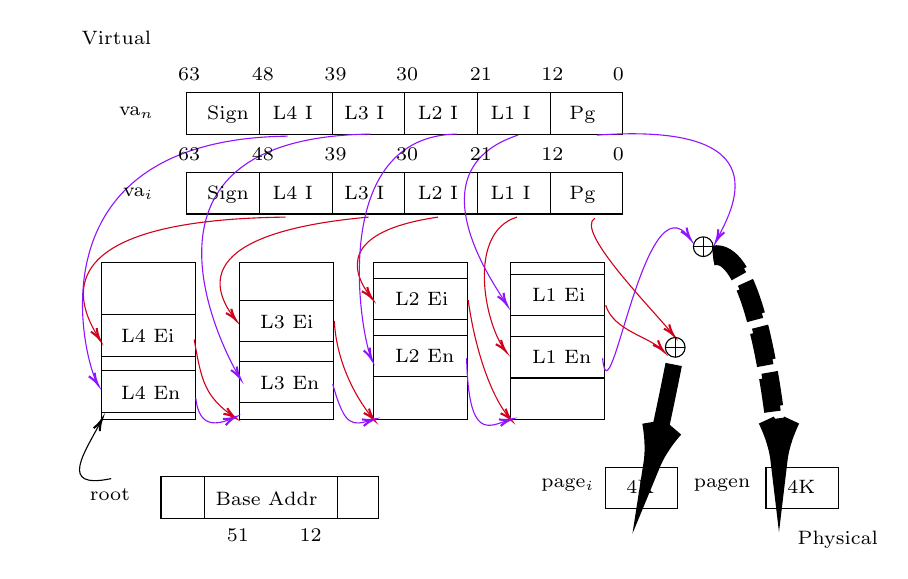
\begin{tikzpicture}[x=0.75pt,y=0.75pt,yscale=-0.5,xscale=0.5]
%uncomment if require: \path (0,532); %set diagram left start at 0, and has height of 532

%Shape: Rectangle [id:dp9406932326447903] 
\draw   (33,240) -- (123,240) -- (123,391) -- (33,391) -- cycle ;
%Shape: Rectangle [id:dp7682116051394419] 
\draw   (166,240) -- (256,240) -- (256,391) -- (166,391) -- cycle ;
%Shape: Rectangle [id:dp07376733516930423] 
\draw   (295,240) -- (385,240) -- (385,391) -- (295,391) -- cycle ;
%Shape: Rectangle [id:dp7106629147891306] 
\draw   (427,240) -- (517,240) -- (517,391) -- (427,391) -- cycle ;
%Shape: Rectangle [id:dp1342906826203598] 
\draw   (115,153) -- (185,153) -- (185,193) -- (115,193) -- cycle ;
%Shape: Rectangle [id:dp08072439007207399] 
\draw   (185,153) -- (255,153) -- (255,193) -- (185,193) -- cycle ;
%Shape: Rectangle [id:dp8282933603833216] 
\draw   (255,153) -- (325,153) -- (325,193) -- (255,193) -- cycle ;
%Shape: Rectangle [id:dp8416255090865326] 
\draw   (325,153) -- (395,153) -- (395,193) -- (325,193) -- cycle ;
%Shape: Rectangle [id:dp22911958218529804] 
\draw   (395,153) -- (465,153) -- (465,193) -- (395,193) -- cycle ;
%Shape: Rectangle [id:dp33732955213990756] 
\draw   (465,153) -- (535,153) -- (535,193) -- (465,193) -- cycle ;
%Shape: Rectangle [id:dp6628879501744147] 
\draw   (518,437) -- (588,437) -- (588,477) -- (518,477) -- cycle ;
%Curve Lines [id:da6688730321284677] 
\draw [color={rgb, 255:red, 208; green, 2; blue, 27 }  ,draw opacity=1 ]   (210,196) .. controls (-37.94,198.94) and (15.69,289.28) .. (30.17,312.65) ;
\draw [shift={(31,314)}, rotate = 238.24] [color={rgb, 255:red, 208; green, 2; blue, 27 }  ,draw opacity=1 ][line width=0.75]    (10.93,-3.29) .. controls (6.95,-1.4) and (3.31,-0.3) .. (0,0) .. controls (3.31,0.3) and (6.95,1.4) .. (10.93,3.29)   ;
%Shape: Rectangle [id:dp6044747978986409] 
\draw   (33,290) -- (123,290) -- (123,330) -- (33,330) -- cycle ;
%Curve Lines [id:da8867562998134584] 
\draw [color={rgb, 255:red, 208; green, 2; blue, 27 }  ,draw opacity=1 ]   (290,196) .. controls (116.54,211.68) and (140.92,267.7) .. (160.79,293.46) ;
\draw [shift={(162,295)}, rotate = 231.34] [color={rgb, 255:red, 208; green, 2; blue, 27 }  ,draw opacity=1 ][line width=0.75]    (10.93,-3.29) .. controls (6.95,-1.4) and (3.31,-0.3) .. (0,0) .. controls (3.31,0.3) and (6.95,1.4) .. (10.93,3.29)   ;
%Shape: Rectangle [id:dp8861153167245819] 
\draw   (166,276) -- (256,276) -- (256,316) -- (166,316) -- cycle ;
%Shape: Rectangle [id:dp05979844200848894] 
\draw   (295,255) -- (385,255) -- (385,295) -- (295,295) -- cycle ;
%Shape: Rectangle [id:dp17403733244247843] 
\draw   (427,311) -- (517,311) -- (517,351) -- (427,351) -- cycle ;
%Curve Lines [id:da20581124900573955] 
\draw [color={rgb, 255:red, 208; green, 2; blue, 27 }  ,draw opacity=1 ]   (357,196) .. controls (262.92,209.72) and (272.56,247.45) .. (291.81,272.48) ;
\draw [shift={(293,274)}, rotate = 231.34] [color={rgb, 255:red, 208; green, 2; blue, 27 }  ,draw opacity=1 ][line width=0.75]    (10.93,-3.29) .. controls (6.95,-1.4) and (3.31,-0.3) .. (0,0) .. controls (3.31,0.3) and (6.95,1.4) .. (10.93,3.29)   ;
%Curve Lines [id:da07589611603635316] 
\draw [color={rgb, 255:red, 208; green, 2; blue, 27 }  ,draw opacity=1 ]   (433,196) .. controls (384.98,210.7) and (401.31,296.47) .. (420.8,323.42) ;
\draw [shift={(422,325)}, rotate = 231.34] [color={rgb, 255:red, 208; green, 2; blue, 27 }  ,draw opacity=1 ][line width=0.75]    (10.93,-3.29) .. controls (6.95,-1.4) and (3.31,-0.3) .. (0,0) .. controls (3.31,0.3) and (6.95,1.4) .. (10.93,3.29)   ;
%Curve Lines [id:da6852167546673456] 
\draw [color={rgb, 255:red, 208; green, 2; blue, 27 }  ,draw opacity=1 ]   (508,197) .. controls (488.3,208.82) and (561.74,282.73) .. (583.06,308.84) ;
\draw [shift={(584,310)}, rotate = 231.34] [color={rgb, 255:red, 208; green, 2; blue, 27 }  ,draw opacity=1 ][line width=0.75]    (10.93,-3.29) .. controls (6.95,-1.4) and (3.31,-0.3) .. (0,0) .. controls (3.31,0.3) and (6.95,1.4) .. (10.93,3.29)   ;
%Curve Lines [id:da6285305490382367] 
\draw [color={rgb, 255:red, 0; green, 0; blue, 0 }  ,draw opacity=1 ][line width=6]    (584,338) .. controls (581.75,349.7) and (571.81,399.47) .. (564.74,427.53) ;
\draw [shift={(562.5,436)}, rotate = 285.64] [color={rgb, 255:red, 0; green, 0; blue, 0 }  ,draw opacity=1 ][line width=6]    (40.44,-12.17) .. controls (25.71,-5.16) and (12.23,-1.11) .. (0,0) .. controls (12.23,1.11) and (25.71,5.17) .. (40.44,12.17)   ;
%Curve Lines [id:da017521077423665377] 
\draw    (42,448) .. controls (-10.21,458.84) and (17.15,422.13) .. (32.32,392.36) ;
\draw [shift={(33,391)}, rotate = 116.57] [color={rgb, 255:red, 0; green, 0; blue, 0 }  ][line width=0.75]    (10.93,-3.29) .. controls (6.95,-1.4) and (3.31,-0.3) .. (0,0) .. controls (3.31,0.3) and (6.95,1.4) .. (10.93,3.29)   ;
%Curve Lines [id:da6750042432035159] 
\draw [color={rgb, 255:red, 208; green, 2; blue, 27 }  ,draw opacity=1 ]   (122,314) .. controls (128.9,353.4) and (131.91,368.54) .. (159.71,388.1) ;
\draw [shift={(161,389)}, rotate = 214.59] [color={rgb, 255:red, 208; green, 2; blue, 27 }  ,draw opacity=1 ][line width=0.75]    (10.93,-3.29) .. controls (6.95,-1.4) and (3.31,-0.3) .. (0,0) .. controls (3.31,0.3) and (6.95,1.4) .. (10.93,3.29)   ;
%Curve Lines [id:da14788158682113428] 
\draw [color={rgb, 255:red, 208; green, 2; blue, 27 }  ,draw opacity=1 ]   (257,296) .. controls (258.95,335) and (277.06,369.25) .. (293.72,389.47) ;
\draw [shift={(295,391)}, rotate = 229.64] [color={rgb, 255:red, 208; green, 2; blue, 27 }  ,draw opacity=1 ][line width=0.75]    (10.93,-3.29) .. controls (6.95,-1.4) and (3.31,-0.3) .. (0,0) .. controls (3.31,0.3) and (6.95,1.4) .. (10.93,3.29)   ;
%Curve Lines [id:da3297977595767969] 
\draw [color={rgb, 255:red, 208; green, 2; blue, 27 }  ,draw opacity=1 ]   (386,276) .. controls (392.86,325) and (408.36,369.2) .. (425.92,389.77) ;
\draw [shift={(427,391)}, rotate = 228.01] [color={rgb, 255:red, 208; green, 2; blue, 27 }  ,draw opacity=1 ][line width=0.75]    (10.93,-3.29) .. controls (6.95,-1.4) and (3.31,-0.3) .. (0,0) .. controls (3.31,0.3) and (6.95,1.4) .. (10.93,3.29)   ;
%Curve Lines [id:da7710391961792686] 
\draw [color={rgb, 255:red, 208; green, 2; blue, 27 }  ,draw opacity=1 ]   (518.5,281) .. controls (526.26,305.25) and (558.95,310.68) .. (572.77,323.76) ;
\draw [shift={(574,325)}, rotate = 227.12] [color={rgb, 255:red, 208; green, 2; blue, 27 }  ,draw opacity=1 ][line width=0.75]    (10.93,-3.29) .. controls (6.95,-1.4) and (3.31,-0.3) .. (0,0) .. controls (3.31,0.3) and (6.95,1.4) .. (10.93,3.29)   ;
%Shape: Rectangle [id:dp8163096906532217] 
\draw   (115,76) -- (185,76) -- (185,116) -- (115,116) -- cycle ;
%Shape: Rectangle [id:dp5008947189169124] 
\draw   (185,76) -- (255,76) -- (255,116) -- (185,116) -- cycle ;
%Shape: Rectangle [id:dp20199565750745574] 
\draw   (255,76) -- (325,76) -- (325,116) -- (255,116) -- cycle ;
%Shape: Rectangle [id:dp6456722127145564] 
\draw   (325,76) -- (395,76) -- (395,116) -- (325,116) -- cycle ;
%Shape: Rectangle [id:dp2840441308370316] 
\draw   (395,76) -- (465,76) -- (465,116) -- (395,116) -- cycle ;
%Shape: Rectangle [id:dp8377187529278063] 
\draw   (465,76) -- (535,76) -- (535,116) -- (465,116) -- cycle ;
%Shape: Rectangle [id:dp8211934221770631] 
\draw   (33,344) -- (123,344) -- (123,384) -- (33,384) -- cycle ;
%Shape: Rectangle [id:dp8913167857456976] 
\draw   (166,335) -- (256,335) -- (256,375) -- (166,375) -- cycle ;
%Shape: Rectangle [id:dp9695091175432768] 
\draw   (295,310) -- (385,310) -- (385,350) -- (295,350) -- cycle ;
%Shape: Rectangle [id:dp6695852511595983] 
\draw   (427,251) -- (517,251) -- (517,291) -- (427,291) -- cycle ;
%Shape: Rectangle [id:dp7443372414988962] 
\draw   (673,437) -- (743,437) -- (743,477) -- (673,477) -- cycle ;
%Curve Lines [id:da8585420033251991] 
\draw [color={rgb, 255:red, 144; green, 19; blue, 254 }  ,draw opacity=1 ]   (212,118) .. controls (-35.94,120.94) and (13.84,327.48) .. (28.17,355.51) ;
\draw [shift={(29,357)}, rotate = 238.24] [color={rgb, 255:red, 144; green, 19; blue, 254 }  ,draw opacity=1 ][line width=0.75]    (10.93,-3.29) .. controls (6.95,-1.4) and (3.31,-0.3) .. (0,0) .. controls (3.31,0.3) and (6.95,1.4) .. (10.93,3.29)   ;
%Curve Lines [id:da3950862908580315] 
\draw [color={rgb, 255:red, 144; green, 19; blue, 254 }  ,draw opacity=1 ]   (292,116) .. controls (44.06,118.94) and (148.59,321.64) .. (165.1,349.52) ;
\draw [shift={(166,351)}, rotate = 238.24] [color={rgb, 255:red, 144; green, 19; blue, 254 }  ,draw opacity=1 ][line width=0.75]    (10.93,-3.29) .. controls (6.95,-1.4) and (3.31,-0.3) .. (0,0) .. controls (3.31,0.3) and (6.95,1.4) .. (10.93,3.29)   ;
%Curve Lines [id:da33073679964999325] 
\draw [color={rgb, 255:red, 144; green, 19; blue, 254 }  ,draw opacity=1 ]   (375,116) .. controls (252.5,117.96) and (280.78,302.4) .. (292.32,331.42) ;
\draw [shift={(293,333)}, rotate = 244.44] [color={rgb, 255:red, 144; green, 19; blue, 254 }  ,draw opacity=1 ][line width=0.75]    (10.93,-3.29) .. controls (6.95,-1.4) and (3.31,-0.3) .. (0,0) .. controls (3.31,0.3) and (6.95,1.4) .. (10.93,3.29)   ;
%Curve Lines [id:da8024795963071514] 
\draw [color={rgb, 255:red, 144; green, 19; blue, 254 }  ,draw opacity=1 ]   (434,117) .. controls (333.57,150.15) and (408.07,256.5) .. (422.05,278.48) ;
\draw [shift={(423,280)}, rotate = 238.57] [color={rgb, 255:red, 144; green, 19; blue, 254 }  ,draw opacity=1 ][line width=0.75]    (10.93,-3.29) .. controls (6.95,-1.4) and (3.31,-0.3) .. (0,0) .. controls (3.31,0.3) and (6.95,1.4) .. (10.93,3.29)   ;
%Curve Lines [id:da02032635448677178] 
\draw [color={rgb, 255:red, 144; green, 19; blue, 254 }  ,draw opacity=1 ]   (510,117) .. controls (690.32,104.26) and (640.14,189.48) .. (625.83,217.37) ;
\draw [shift={(625,219)}, rotate = 296.57] [color={rgb, 255:red, 144; green, 19; blue, 254 }  ,draw opacity=1 ][line width=0.75]    (10.93,-3.29) .. controls (6.95,-1.4) and (3.31,-0.3) .. (0,0) .. controls (3.31,0.3) and (6.95,1.4) .. (10.93,3.29)   ;
%Curve Lines [id:da41060712415524825] 
\draw [color={rgb, 255:red, 0; green, 0; blue, 0 }  ,draw opacity=1 ][line width=6]  [dash pattern={on 12.38pt off 4.5pt}]  (621.68,231.53) .. controls (622.92,231.26) and (624.14,231.13) .. (625.34,231.13) .. controls (633.77,231.13) and (641.39,237.71) .. (648.05,248.98) .. controls (659.27,267.99) and (667.85,300.17) .. (674.03,332.37) .. controls (681.19,369.64) and (685.18,406.91) .. (686,417.65)(622.32,234.47) .. controls (623.34,234.24) and (624.35,234.13) .. (625.34,234.13) .. controls (632.96,234.13) and (639.57,240.52) .. (645.47,250.5) .. controls (656.56,269.29) and (664.97,301.12) .. (671.09,332.94) .. controls (678.22,370.07) and (682.2,407.21) .. (683.01,417.91) ;
\draw [shift={(685.5,432)}, rotate = 270] [color={rgb, 255:red, 0; green, 0; blue, 0 }  ,draw opacity=1 ][line width=6]    (40.44,-12.17) .. controls (25.71,-5.16) and (12.23,-1.11) .. (0,0) .. controls (12.23,1.11) and (25.71,5.17) .. (40.44,12.17)   ;
%Curve Lines [id:da15754024469049188] 
\draw [color={rgb, 255:red, 144; green, 19; blue, 254 }  ,draw opacity=1 ]   (123.5,370) .. controls (126.4,399.92) and (144.19,396.31) .. (159.36,389.73) ;
\draw [shift={(161,389)}, rotate = 155.7] [color={rgb, 255:red, 144; green, 19; blue, 254 }  ,draw opacity=1 ][line width=0.75]    (10.93,-3.29) .. controls (6.95,-1.4) and (3.31,-0.3) .. (0,0) .. controls (3.31,0.3) and (6.95,1.4) .. (10.93,3.29)   ;
%Curve Lines [id:da2801023256877153] 
\draw [color={rgb, 255:red, 144; green, 19; blue, 254 }  ,draw opacity=1 ]   (255.5,357) .. controls (267.14,398.71) and (274.08,397.14) .. (293.19,391.53) ;
\draw [shift={(295,391)}, rotate = 163.69] [color={rgb, 255:red, 144; green, 19; blue, 254 }  ,draw opacity=1 ][line width=0.75]    (10.93,-3.29) .. controls (6.95,-1.4) and (3.31,-0.3) .. (0,0) .. controls (3.31,0.3) and (6.95,1.4) .. (10.93,3.29)   ;
%Curve Lines [id:da5373695051918006] 
\draw [color={rgb, 255:red, 144; green, 19; blue, 254 }  ,draw opacity=1 ]   (384.5,332) .. controls (386.44,411.54) and (405.32,397.93) .. (425.16,391.57) ;
\draw [shift={(427,391)}, rotate = 163.69] [color={rgb, 255:red, 144; green, 19; blue, 254 }  ,draw opacity=1 ][line width=0.75]    (10.93,-3.29) .. controls (6.95,-1.4) and (3.31,-0.3) .. (0,0) .. controls (3.31,0.3) and (6.95,1.4) .. (10.93,3.29)   ;
%Curve Lines [id:da8840761934459798] 
\draw [color={rgb, 255:red, 144; green, 19; blue, 254 }  ,draw opacity=1 ]   (515.5,332) .. controls (522.47,399.66) and (555.67,155.46) .. (599.34,216.06) ;
\draw [shift={(600,217)}, rotate = 235.49] [color={rgb, 255:red, 144; green, 19; blue, 254 }  ,draw opacity=1 ][line width=0.75]    (10.93,-3.29) .. controls (6.95,-1.4) and (3.31,-0.3) .. (0,0) .. controls (3.31,0.3) and (6.95,1.4) .. (10.93,3.29)   ;
%Shape: Rectangle [id:dp967281283756027] 
\draw   (90,446) -- (131.5,446) -- (131.5,486) -- (90,486) -- cycle ;
%Shape: Rectangle [id:dp6818362650206453] 
\draw   (131.5,446) -- (260.5,446) -- (260.5,486) -- (131.5,486) -- cycle ;
%Shape: Rectangle [id:dp6367652388585874] 
\draw   (260.5,446) -- (300,446) -- (300,486) -- (260.5,486) -- cycle ;
\draw   (576,321.5) .. controls (576,316.25) and (580.25,312) .. (585.5,312) .. controls (590.75,312) and (595,316.25) .. (595,321.5) .. controls (595,326.75) and (590.75,331) .. (585.5,331) .. controls (580.25,331) and (576,326.75) .. (576,321.5) -- cycle ; \draw   (576,321.5) -- (595,321.5) ; \draw   (585.5,312) -- (585.5,331) ;
\draw   (603,224.5) .. controls (603,219.25) and (607.25,215) .. (612.5,215) .. controls (617.75,215) and (622,219.25) .. (622,224.5) .. controls (622,229.75) and (617.75,234) .. (612.5,234) .. controls (607.25,234) and (603,229.75) .. (603,224.5) -- cycle ; \draw   (603,224.5) -- (622,224.5) ; \draw   (612.5,215) -- (612.5,234) ;

% Text Node
\draw (11,14) node [anchor=north west][inner sep=0.75pt]   [align=left] {{\scriptsize Virtual}};
% Text Node
\draw (701,496) node [anchor=north west][inner sep=0.75pt]   [align=left] {{\scriptsize Physical}};
% Text Node
\draw (104,127) node [anchor=north west][inner sep=0.75pt]   [align=left] {{\scriptsize 63}};
% Text Node
\draw (175,127) node [anchor=north west][inner sep=0.75pt]   [align=left] {{\scriptsize 48}};
% Text Node
\draw (245,127) node [anchor=north west][inner sep=0.75pt]   [align=left] {{\scriptsize 39}};
% Text Node
\draw (314,127) node [anchor=north west][inner sep=0.75pt]   [align=left] {{\scriptsize 30}};
% Text Node
\draw (385,127) node [anchor=north west][inner sep=0.75pt]   [align=left] {{\scriptsize 21}};
% Text Node
\draw (454,127) node [anchor=north west][inner sep=0.75pt]   [align=left] {{\scriptsize 12}};
% Text Node
\draw (523,127) node [anchor=north west][inner sep=0.75pt]   [align=left] {{\scriptsize 0}};
% Text Node
\draw (132,164) node [anchor=north west][inner sep=0.75pt]   [align=left] {{\scriptsize Sign}};
% Text Node
\draw (195,164) node [anchor=north west][inner sep=0.75pt]   [align=left] {{\scriptsize L4 I}};
% Text Node
\draw (264,164) node [anchor=north west][inner sep=0.75pt]   [align=left] {{\scriptsize L3 I}};
% Text Node
\draw (335,164) node [anchor=north west][inner sep=0.75pt]   [align=left] {{\scriptsize L2 I}};
% Text Node
\draw (405,164) node [anchor=north west][inner sep=0.75pt]   [align=left] {{\scriptsize L1 I}};
% Text Node
\draw (481,164) node [anchor=north west][inner sep=0.75pt]   [align=left] {{\scriptsize Pg}};
% Text Node
\draw (51,166) node [anchor=north west][inner sep=0.75pt]   [align=left] {{\scriptsize va$_i$}};
% Text Node
\draw (19,455) node [anchor=north west][inner sep=0.75pt]   [align=left] {{\scriptsize root}};
% Text Node
\draw (454,446) node [anchor=north west][inner sep=0.75pt]   [align=left] {{\scriptsize page$_i$}};
% Text Node
\draw (536,447) node [anchor=north west][inner sep=0.75pt]   [align=left] {{\scriptsize 4K}};
% Text Node
\draw (49,302) node [anchor=north west][inner sep=0.75pt]   [align=left] {{\scriptsize L4 Ei}};
% Text Node
\draw (183,288) node [anchor=north west][inner sep=0.75pt]   [align=left] {{\scriptsize L3 Ei}};
% Text Node
\draw (313,266) node [anchor=north west][inner sep=0.75pt]   [align=left] {{\scriptsize L2 Ei}};
% Text Node
\draw (445,322) node [anchor=north west][inner sep=0.75pt]   [align=left] {{\scriptsize L1 En}};
% Text Node
\draw (104,50) node [anchor=north west][inner sep=0.75pt]   [align=left] {{\scriptsize 63}};
% Text Node
\draw (175,50) node [anchor=north west][inner sep=0.75pt]   [align=left] {{\scriptsize 48}};
% Text Node
\draw (245,50) node [anchor=north west][inner sep=0.75pt]   [align=left] {{\scriptsize 39}};
% Text Node
\draw (314,50) node [anchor=north west][inner sep=0.75pt]   [align=left] {{\scriptsize 30}};
% Text Node
\draw (385,50) node [anchor=north west][inner sep=0.75pt]   [align=left] {{\scriptsize 21}};
% Text Node
\draw (454,50) node [anchor=north west][inner sep=0.75pt]   [align=left] {{\scriptsize 12}};
% Text Node
\draw (523,50) node [anchor=north west][inner sep=0.75pt]   [align=left] {{\scriptsize 0}};
% Text Node
\draw (132,87) node [anchor=north west][inner sep=0.75pt]   [align=left] {{\scriptsize Sign}};
% Text Node
\draw (195,87) node [anchor=north west][inner sep=0.75pt]   [align=left] {{\scriptsize L4 I}};
% Text Node
\draw (264,87) node [anchor=north west][inner sep=0.75pt]   [align=left] {{\scriptsize L3 I}};
% Text Node
\draw (335,87) node [anchor=north west][inner sep=0.75pt]   [align=left] {{\scriptsize L2 I}};
% Text Node
\draw (405,87) node [anchor=north west][inner sep=0.75pt]   [align=left] {{\scriptsize L1 I}};
% Text Node
\draw (481,87) node [anchor=north west][inner sep=0.75pt]   [align=left] {{\scriptsize Pg}};
% Text Node
\draw (47,88) node [anchor=north west][inner sep=0.75pt]   [align=left] {{\scriptsize va$_n$}};
% Text Node
\draw (49,356) node [anchor=north west][inner sep=0.75pt]   [align=left] {{\scriptsize L4 En}};
% Text Node
\draw (183,347) node [anchor=north west][inner sep=0.75pt]   [align=left] {{\scriptsize L3 En}};
% Text Node
\draw (313,321) node [anchor=north west][inner sep=0.75pt]   [align=left] {{\scriptsize L2 En}};
% Text Node
\draw (445,262) node [anchor=north west][inner sep=0.75pt]   [align=left] {{\scriptsize L1 Ei}};
% Text Node
\draw (601,446) node [anchor=north west][inner sep=0.75pt]   [align=left] {{\scriptsize pagen}};
% Text Node
\draw (691,447) node [anchor=north west][inner sep=0.75pt]   [align=left] {{\scriptsize 4K}};
% Text Node
\draw (151,494) node [anchor=north west][inner sep=0.75pt]   [align=left] {{\scriptsize 51}};
% Text Node
\draw (221,494) node [anchor=north west][inner sep=0.75pt]   [align=left] {{\scriptsize 12}};
% Text Node
\draw (140,458) node [anchor=north west][inner sep=0.75pt]   [align=left] {{\scriptsize Base Addr}};


\end{tikzpicture}
     %  \caption{Bs}
      %  \label{fig:enter-label}
    \end{figure}
    \column{0.30\textwidth}
    \begin{alertblock}{Soundness of Traversal}
    Any update on the \emph{shared page-tables}, which themselves are referenced with \emph{physical memory} addresses, would break the soundness of any other traversal!
    \end{alertblock}
    \end{columns}
\end{frame}
\subsection{Address-Space Agnostic Virtual Memory References}
\begin{frame}{Managing Agnostic Memory Mappings}
    \begin{figure}
        \centering




\tikzset{every picture/.style={line width=0.75pt}} %set default line width to 0.75pt        

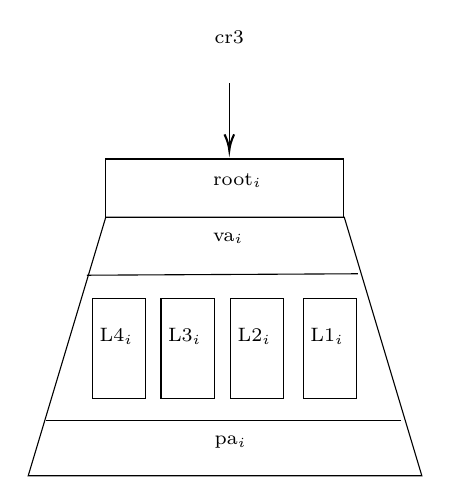
\begin{tikzpicture}[x=0.75pt,y=0.75pt,yscale=-0.7,xscale=0.7]
%uncomment if require: \path (0,444); %set diagram left start at 0, and has height of 444

%Straight Lines [id:da6068809865252034] 
\draw    (179,78) -- (179,122) ;
\draw [shift={(179,124)}, rotate = 270] [color={rgb, 255:red, 0; green, 0; blue, 0 }  ][line width=0.75]    (10.93,-3.29) .. controls (6.95,-1.4) and (3.31,-0.3) .. (0,0) .. controls (3.31,0.3) and (6.95,1.4) .. (10.93,3.29)   ;
%Shape: Trapezoid [id:dp3739735856439024] 
\draw   (40.6,348) -- (94,170) -- (258.1,170) -- (311.5,348) -- cycle ;
%Shape: Rectangle [id:dp6026336395414527] 
\draw   (94,130) -- (257.5,130) -- (257.5,170) -- (94,170) -- cycle ;
%Straight Lines [id:da32976073844810716] 
\draw    (81,210) -- (267.5,209) ;
%Straight Lines [id:da4667182831758503] 
\draw    (53,310) -- (297.5,310) ;
%Shape: Rectangle [id:dp3480638833922085] 
\draw   (85,226) -- (121.5,226) -- (121.5,295) -- (85,295) -- cycle ;
%Shape: Rectangle [id:dp558691590623291] 
\draw   (132,226) -- (168.5,226) -- (168.5,295) -- (132,295) -- cycle ;
%Shape: Rectangle [id:dp5224364674753033] 
\draw   (180,226) -- (216.5,226) -- (216.5,295) -- (180,295) -- cycle ;
%Shape: Rectangle [id:dp7593362242110164] 
\draw   (230,226) -- (266.5,226) -- (266.5,295) -- (230,295) -- cycle ;

% Text Node
\draw (167,40) node [anchor=north west][inner sep=0.75pt]   [align=left] {{\scriptsize cr3}};
% Text Node
\draw (166,179) node [anchor=north west][inner sep=0.75pt]   [align=left] {{\scriptsize va$_i$}};
% Text Node
\draw (167,319) node [anchor=north west][inner sep=0.75pt]   [align=left] {{\scriptsize pa$_i$}};
% Text Node
\draw (88,245) node [anchor=north west][inner sep=0.75pt]   [align=left] {{\scriptsize L4$_i$}};
% Text Node
\draw (166,138) node [anchor=north west][inner sep=0.75pt]   [align=left] {{\scriptsize root$_i$}};
% Text Node
\draw (135,245) node [anchor=north west][inner sep=0.75pt]   [align=left] {{\scriptsize L3$_i$}};
% Text Node
\draw (183,245) node [anchor=north west][inner sep=0.75pt]   [align=left] {{\scriptsize L2$_i$}};
% Text Node
\draw (233,245) node [anchor=north west][inner sep=0.75pt]   [align=left] {{\scriptsize L1$_i$}};


\end{tikzpicture}
        \caption{An Address Space with Unique Root Address \textsf{root}$_i$}
        \label{fig:enter-label}
    \end{figure}
\end{frame}
\begin{frame}{Managing Agnostic Memory Mappings}
    \begin{figure}
        \centering
        


\tikzset{every picture/.style={line width=0.75pt}} %set default line width to 0.75pt        

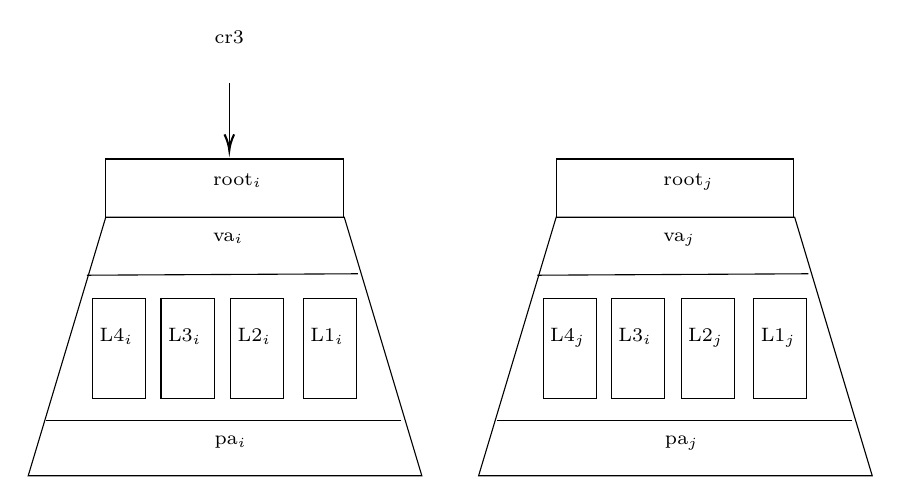
\begin{tikzpicture}[x=0.75pt,y=0.75pt,yscale=-0.7,xscale=0.7]
%uncomment if require: \path (0,444); %set diagram left start at 0, and has height of 444

%Straight Lines [id:da6068809865252034] 
\draw    (179,78) -- (179,122) ;
\draw [shift={(179,124)}, rotate = 270] [color={rgb, 255:red, 0; green, 0; blue, 0 }  ][line width=0.75]    (10.93,-3.29) .. controls (6.95,-1.4) and (3.31,-0.3) .. (0,0) .. controls (3.31,0.3) and (6.95,1.4) .. (10.93,3.29)   ;
%Shape: Trapezoid [id:dp3739735856439024] 
\draw   (40.6,348) -- (94,170) -- (258.1,170) -- (311.5,348) -- cycle ;
%Shape: Rectangle [id:dp6026336395414527] 
\draw   (94,130) -- (257.5,130) -- (257.5,170) -- (94,170) -- cycle ;
%Straight Lines [id:da32976073844810716] 
\draw    (81,210) -- (267.5,209) ;
%Straight Lines [id:da4667182831758503] 
\draw    (53,310) -- (297.5,310) ;
%Shape: Rectangle [id:dp3480638833922085] 
\draw   (85,226) -- (121.5,226) -- (121.5,295) -- (85,295) -- cycle ;
%Shape: Rectangle [id:dp558691590623291] 
\draw   (132,226) -- (168.5,226) -- (168.5,295) -- (132,295) -- cycle ;
%Shape: Rectangle [id:dp5224364674753033] 
\draw   (180,226) -- (216.5,226) -- (216.5,295) -- (180,295) -- cycle ;
%Shape: Rectangle [id:dp7593362242110164] 
\draw   (230,226) -- (266.5,226) -- (266.5,295) -- (230,295) -- cycle ;
%Shape: Trapezoid [id:dp17680532195155196] 
\draw   (350.6,348) -- (404,170) -- (568.1,170) -- (621.5,348) -- cycle ;
%Shape: Rectangle [id:dp1391273388270049] 
\draw   (404,130) -- (567.5,130) -- (567.5,170) -- (404,170) -- cycle ;
%Straight Lines [id:da16412176418294644] 
\draw    (391,210) -- (577.5,209) ;
%Straight Lines [id:da02392113930828521] 
\draw    (363,310) -- (607.5,310) ;
%Shape: Rectangle [id:dp3343779414527479] 
\draw   (395,226) -- (431.5,226) -- (431.5,295) -- (395,295) -- cycle ;
%Shape: Rectangle [id:dp5031533033051587] 
\draw   (442,226) -- (478.5,226) -- (478.5,295) -- (442,295) -- cycle ;
%Shape: Rectangle [id:dp6176432721746983] 
\draw   (490,226) -- (526.5,226) -- (526.5,295) -- (490,295) -- cycle ;
%Shape: Rectangle [id:dp8967436529993302] 
\draw   (540,226) -- (576.5,226) -- (576.5,295) -- (540,295) -- cycle ;

% Text Node
\draw (167,40) node [anchor=north west][inner sep=0.75pt]   [align=left] {{\scriptsize cr3}};
% Text Node
\draw (166,179) node [anchor=north west][inner sep=0.75pt]   [align=left] {{\scriptsize va$_i$}};
% Text Node
\draw (167,319) node [anchor=north west][inner sep=0.75pt]   [align=left] {{\scriptsize pa$_i$}};
% Text Node
\draw (88,245) node [anchor=north west][inner sep=0.75pt]   [align=left] {{\scriptsize L4$_i$}};
% Text Node
\draw (166,138) node [anchor=north west][inner sep=0.75pt]   [align=left] {{\scriptsize root$_i$}};
% Text Node
\draw (135,245) node [anchor=north west][inner sep=0.75pt]   [align=left] {{\scriptsize L3$_i$}};
% Text Node
\draw (183,245) node [anchor=north west][inner sep=0.75pt]   [align=left] {{\scriptsize L2$_i$}};
% Text Node
\draw (233,245) node [anchor=north west][inner sep=0.75pt]   [align=left] {{\scriptsize L1$_i$}};
% Text Node
\draw (476,179) node [anchor=north west][inner sep=0.75pt]   [align=left] {{\scriptsize va$_j$}};
% Text Node
\draw (477,319) node [anchor=north west][inner sep=0.75pt]   [align=left] {{\scriptsize pa$_j$}};
% Text Node
\draw (398,245) node [anchor=north west][inner sep=0.75pt]   [align=left] {{\scriptsize L4$_j$}};
% Text Node
\draw (476,138) node [anchor=north west][inner sep=0.75pt]   [align=left] {{\scriptsize root$_j$}};
% Text Node
\draw (445,245) node [anchor=north west][inner sep=0.75pt]   [align=left] {{\scriptsize L3$_i$}};
% Text Node
\draw (493,245) node [anchor=north west][inner sep=0.75pt]   [align=left] {{\scriptsize L2$_j$}};
% Text Node
\draw (543,245) node [anchor=north west][inner sep=0.75pt]   [align=left] {{\scriptsize L1$_j$}};


\end{tikzpicture}
        \caption{Two Address-Spaces with the Unique Root Addresses \textsf{root}$_i$ and \textsf{root}$_j$}
        \label{fig:enter-label}
    \end{figure}
   
\end{frame}
\begin{frame}{Managing Agnostic Memory Mappings}
    \begin{figure}
        \centering
        


\tikzset{every picture/.style={line width=0.75pt}} %set default line width to 0.75pt        

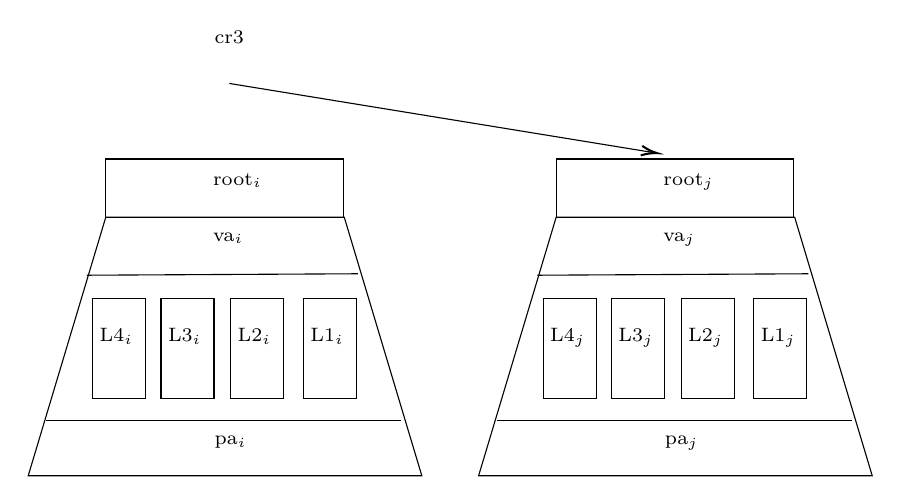
\begin{tikzpicture}[x=0.75pt,y=0.75pt,yscale=-0.7,xscale=0.7]
%uncomment if require: \path (0,444); %set diagram left start at 0, and has height of 444

%Straight Lines [id:da38505936382975436] 
\draw    (186,98) -- (478.53,145.68) ;
\draw [shift={(480.5,146)}, rotate = 189.26] [color={rgb, 255:red, 0; green, 0; blue, 0 }  ][line width=0.75]    (10.93,-3.29) .. controls (6.95,-1.4) and (3.31,-0.3) .. (0,0) .. controls (3.31,0.3) and (6.95,1.4) .. (10.93,3.29)   ;
%Shape: Trapezoid [id:dp7414076994636136] 
\draw   (47.6,368) -- (101,190) -- (265.1,190) -- (318.5,368) -- cycle ;
%Shape: Rectangle [id:dp6682076995791875] 
\draw   (101,150) -- (264.5,150) -- (264.5,190) -- (101,190) -- cycle ;
%Straight Lines [id:da13111570073586742] 
\draw    (88,230) -- (274.5,229) ;
%Straight Lines [id:da8088550891516297] 
\draw    (60,330) -- (304.5,330) ;
%Shape: Rectangle [id:dp21836577048687023] 
\draw   (92,246) -- (128.5,246) -- (128.5,315) -- (92,315) -- cycle ;
%Shape: Rectangle [id:dp057930941757168064] 
\draw   (139,246) -- (175.5,246) -- (175.5,315) -- (139,315) -- cycle ;
%Shape: Rectangle [id:dp39663188007381556] 
\draw   (187,246) -- (223.5,246) -- (223.5,315) -- (187,315) -- cycle ;
%Shape: Rectangle [id:dp5224337498132685] 
\draw   (237,246) -- (273.5,246) -- (273.5,315) -- (237,315) -- cycle ;
%Shape: Trapezoid [id:dp471852322248028] 
\draw   (357.6,368) -- (411,190) -- (575.1,190) -- (628.5,368) -- cycle ;
%Shape: Rectangle [id:dp5528716184490898] 
\draw   (411,150) -- (574.5,150) -- (574.5,190) -- (411,190) -- cycle ;
%Straight Lines [id:da7602460644496329] 
\draw    (398,230) -- (584.5,229) ;
%Straight Lines [id:da6992377024554963] 
\draw    (370,330) -- (614.5,330) ;
%Shape: Rectangle [id:dp8266326943417694] 
\draw   (402,246) -- (438.5,246) -- (438.5,315) -- (402,315) -- cycle ;
%Shape: Rectangle [id:dp6075494266540686] 
\draw   (449,246) -- (485.5,246) -- (485.5,315) -- (449,315) -- cycle ;
%Shape: Rectangle [id:dp7706384125026737] 
\draw   (497,246) -- (533.5,246) -- (533.5,315) -- (497,315) -- cycle ;
%Shape: Rectangle [id:dp6101896478605242] 
\draw   (547,246) -- (583.5,246) -- (583.5,315) -- (547,315) -- cycle ;

% Text Node
\draw (174,60) node [anchor=north west][inner sep=0.75pt]   [align=left] {{\scriptsize cr3}};
% Text Node
\draw (173,199) node [anchor=north west][inner sep=0.75pt]   [align=left] {{\scriptsize va$_i$}};
% Text Node
\draw (174,339) node [anchor=north west][inner sep=0.75pt]   [align=left] {{\scriptsize pa$_i$}};
% Text Node
\draw (95,265) node [anchor=north west][inner sep=0.75pt]   [align=left] {{\scriptsize L4$_i$}};
% Text Node
\draw (173,158) node [anchor=north west][inner sep=0.75pt]   [align=left] {{\scriptsize root$_i$}};
% Text Node
\draw (142,265) node [anchor=north west][inner sep=0.75pt]   [align=left] {{\scriptsize L3$_i$}};
% Text Node
\draw (190,265) node [anchor=north west][inner sep=0.75pt]   [align=left] {{\scriptsize L2$_i$}};
% Text Node
\draw (240,265) node [anchor=north west][inner sep=0.75pt]   [align=left] {{\scriptsize L1$_i$}};
% Text Node
\draw (483,199) node [anchor=north west][inner sep=0.75pt]   [align=left] {{\scriptsize va$_j$}};
% Text Node
\draw (484,339) node [anchor=north west][inner sep=0.75pt]   [align=left] {{\scriptsize pa$_j$}};
% Text Node
\draw (405,265) node [anchor=north west][inner sep=0.75pt]   [align=left] {{\scriptsize L4$_j$}};
% Text Node
\draw (483,158) node [anchor=north west][inner sep=0.75pt]   [align=left] {{\scriptsize root$_j$}};
% Text Node
\draw (452,265) node [anchor=north west][inner sep=0.75pt]   [align=left] {{\scriptsize L3$_j$}};
% Text Node
\draw (500,265) node [anchor=north west][inner sep=0.75pt]   [align=left] {{\scriptsize L2$_j$}};
% Text Node
\draw (550,265) node [anchor=north west][inner sep=0.75pt]   [align=left] {{\scriptsize L1$_j$}};


\end{tikzpicture}
        \caption{Switching Address-Spaces}
        \label{fig:enter-label}
    \end{figure}
\end{frame}
\begin{frame}{Managing Agnostic Memory Mappings}
\begin{columns}
\column{0.65\textwidth}    
    \begin{figure}
        \centering
\tikzset{every picture/.style={line width=0.75pt}} %set default line width to 0.75pt        

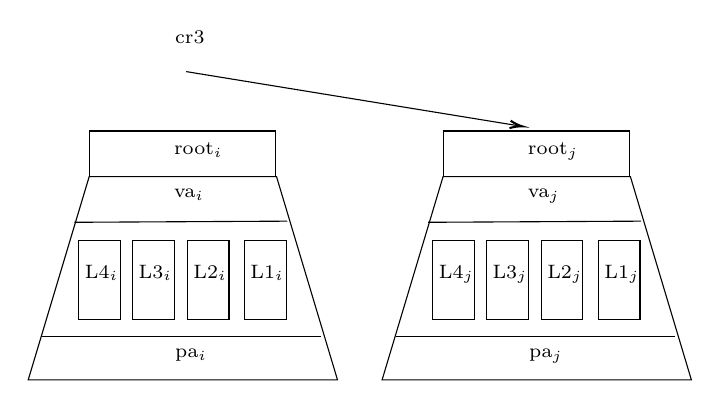
\begin{tikzpicture}[x=0.75pt,y=0.75pt,yscale=-0.55,xscale=0.55]
%uncomment if require: \path (0,444); %set diagram left start at 0, and has height of 444

%Straight Lines [id:da38505936382975436] 
\draw    (186,98) -- (478.53,145.68) ;
\draw [shift={(480.5,146)}, rotate = 189.26] [color={rgb, 255:red, 0; green, 0; blue, 0 }  ][line width=0.75]    (10.93,-3.29) .. controls (6.95,-1.4) and (3.31,-0.3) .. (0,0) .. controls (3.31,0.3) and (6.95,1.4) .. (10.93,3.29)   ;
%Shape: Trapezoid [id:dp7414076994636136] 
\draw   (47.6,368) -- (101,190) -- (265.1,190) -- (318.5,368) -- cycle ;
%Shape: Rectangle [id:dp6682076995791875] 
\draw   (101,150) -- (264.5,150) -- (264.5,190) -- (101,190) -- cycle ;
%Straight Lines [id:da13111570073586742] 
\draw    (88,230) -- (274.5,229) ;
%Straight Lines [id:da8088550891516297] 
\draw    (60,330) -- (304.5,330) ;
%Shape: Rectangle [id:dp21836577048687023] 
\draw   (92,246) -- (128.5,246) -- (128.5,315) -- (92,315) -- cycle ;
%Shape: Rectangle [id:dp057930941757168064] 
\draw   (139,246) -- (175.5,246) -- (175.5,315) -- (139,315) -- cycle ;
%Shape: Rectangle [id:dp39663188007381556] 
\draw   (187,246) -- (223.5,246) -- (223.5,315) -- (187,315) -- cycle ;
%Shape: Rectangle [id:dp5224337498132685] 
\draw   (237,246) -- (273.5,246) -- (273.5,315) -- (237,315) -- cycle ;
%Shape: Trapezoid [id:dp471852322248028] 
\draw   (357.6,368) -- (411,190) -- (575.1,190) -- (628.5,368) -- cycle ;
%Shape: Rectangle [id:dp5528716184490898] 
\draw   (411,150) -- (574.5,150) -- (574.5,190) -- (411,190) -- cycle ;
%Straight Lines [id:da7602460644496329] 
\draw    (398,230) -- (584.5,229) ;
%Straight Lines [id:da6992377024554963] 
\draw    (370,330) -- (614.5,330) ;
%Shape: Rectangle [id:dp8266326943417694] 
\draw   (402,246) -- (438.5,246) -- (438.5,315) -- (402,315) -- cycle ;
%Shape: Rectangle [id:dp6075494266540686] 
\draw   (449,246) -- (485.5,246) -- (485.5,315) -- (449,315) -- cycle ;
%Shape: Rectangle [id:dp7706384125026737] 
\draw   (497,246) -- (533.5,246) -- (533.5,315) -- (497,315) -- cycle ;
%Shape: Rectangle [id:dp6101896478605242] 
\draw   (547,246) -- (583.5,246) -- (583.5,315) -- (547,315) -- cycle ;

% Text Node
\draw (174,60) node [anchor=north west][inner sep=0.75pt]   [align=left] {{\scriptsize cr3}};
% Text Node
\draw (173,199) node [anchor=north west][inner sep=0.75pt]   [align=left] {{\scriptsize va$_i$}};
% Text Node
\draw (174,339) node [anchor=north west][inner sep=0.75pt]   [align=left] {{\scriptsize pa$_i$}};
% Text Node
\draw (95,265) node [anchor=north west][inner sep=0.75pt]   [align=left] {{\scriptsize L4$_i$}};
% Text Node
\draw (173,158) node [anchor=north west][inner sep=0.75pt]   [align=left] {{\scriptsize root$_i$}};
% Text Node
\draw (142,265) node [anchor=north west][inner sep=0.75pt]   [align=left] {{\scriptsize L3$_i$}};
% Text Node
\draw (190,265) node [anchor=north west][inner sep=0.75pt]   [align=left] {{\scriptsize L2$_i$}};
% Text Node
\draw (240,265) node [anchor=north west][inner sep=0.75pt]   [align=left] {{\scriptsize L1$_i$}};
% Text Node
\draw (483,199) node [anchor=north west][inner sep=0.75pt]   [align=left] {{\scriptsize va$_j$}};
% Text Node
\draw (484,339) node [anchor=north west][inner sep=0.75pt]   [align=left] {{\scriptsize pa$_j$}};
% Text Node
\draw (405,265) node [anchor=north west][inner sep=0.75pt]   [align=left] {{\scriptsize L4$_j$}};
% Text Node
\draw (483,158) node [anchor=north west][inner sep=0.75pt]   [align=left] {{\scriptsize root$_j$}};
% Text Node
\draw (452,265) node [anchor=north west][inner sep=0.75pt]   [align=left] {{\scriptsize L3$_j$}};
% Text Node
\draw (500,265) node [anchor=north west][inner sep=0.75pt]   [align=left] {{\scriptsize L2$_j$}};
% Text Node
\draw (550,265) node [anchor=north west][inner sep=0.75pt]   [align=left] {{\scriptsize L1$_j$}};


\end{tikzpicture}
        \caption{Switching Address-Spaces}
        \label{fig:enter-label}
    \end{figure}
     \column{0.375\textwidth}
    \begin{alertblock}{Referring to Agnostic Resources}
    Unless we bookkeep to which address-space each of these virtual-to-physical mappings belongs,  \emph{which we never see in the practice of using virtual memory references}, we need to figure out a way of referring to these mappings as \emph{they are only valid in their own address-spaces}.
    \end{alertblock}
    \end{columns}
\end{frame}
\section{Logic}
\subsection{A Quick Tour on Separation Logic (\textbf{SL})}
\begin{frame}{Specifying Programs}
    \[\{P\}\; C\; \{Q\} \]
\end{frame}
\begin{frame}{Separation Logic: Separating Conjuction}
   \[
\inferrule[Frame]{
	\triple{P}{e}{Q}
}{
	\triple{P\ast R}{e}{Q\ast R}
}
\]
\end{frame}
\begin{frame}{Separation Logic: Ownership}
    \begin{itemize}
        \item Well-known points-to assertion, e.g., $\mathsf{memory\_ref}\; \mapsto_{q} \;\mathsf{val}$
        \item Regarding the logical machinery, Iris \textbf{SL} enables encoding a generalized form ownership of \emph{logical resources}
        \item A fragmental $\ownGhost{\gamma}{P}$ ownership
            \begin{itemize}
            \item Enabling coordinated access to logical resources \end{itemize}
        \item Full $ \fbox{$P$}^\gamma$ ownership 
         \begin{itemize}
            \item Enabling access to \emph{update} logical resources, presented as \emph{invariants}
             \end{itemize}
    \end{itemize}
\end{frame}
\begin{frame}{Separation Logic: Invariants}
\[
    \inferrule[Inv]{
        \triple{  P \ast R }{\alpha}{P \ast Q }_{\epsilon}\\
        \alpha~\textrm{physically atomic}
    }{
        \fbox{$P$}^n \vdash \triple{ R }{\alpha}{ Q }_{\epsilon \uplus \{n\}}
    }
    \]
\end{frame}
\subsection{A Logic for Recovering the Soundness of Page-Table Traversal}
\begin{frame}{Defining Some Ownersip Assertions}
    \begin{itemize}
    \item   Expected to have register ownership to be defined : $\mathsf{reg} \; \mapsto_{r} \; \mathsf{reg\_val}$
        \item Expected to have \emph{physical memory} ownership defined: $\mathsf{pa} \; \mapsto_{p} \; \mathsf{val}$
        \item How about virtual memory references?
    \end{itemize}
\end{frame}
\begin{frame}{A Naive Attempt on Virtual-Pointsto}
    \begin{itemize}
        \item Page and page table addresses are \emph{physical}
        \item Purple (or red) path + bold black page references are \emph{physical}
        \item Why don't we define \emph{virtual} memory references in terms of the physical page-table and the final page references? 
    \end{itemize}
      \[ \textsf{L}_{4}\_\textsf{L}_{1}\_\textsf{PointsTo}(\vaddr\textsf{, l4e, l3e, l2e, l1e, paddr}) + paddr \mapsto_{p} \mathsf{page\_val}\]
% 
\end{frame}
\begin{frame}{Tokens for Traversals} \scriptsize
    \begin{columns}
        \column{0.5\textwidth}
\[        \underbrace{\fracghostmaptoken{\delta}{\vaddr}{\paddr}{\qfrac} }_\text{Ghost translation} \ast \underbrace{\paddr \mapsto_{\mathsf{p}}\{\textsf{qfrac}\}\; \vale}_\text{Physical location} \]
        \column{0.5\textwidth}
        \begin{itemize}
            \item Abstract the purple and red segment of page-table traversal into \emph{logical summarization of the walk}
            \item Distribute the fragmental ownersip of the logical page-table summarization to virtual memory ownership
        \end{itemize}
    \end{columns}
\end{frame}

\begin{frame}{Some Parts from Kernel Invariant}\scriptsize
    \begin{definition}[The Kernel Invariant for Page-Table Traversal with Virtual Page-Table Pointers]
        
\[
\begin{array}{l}
  \mathcal{I}\textsf{ASpace}_{\textsf{id}}(\ptablestore,\Xi,m)\stackrel{\triangle}{=} \textsf{ASpace\_Lookup}_{\textsf{id}}(\ptablestore,\Xi,m) \ast \mathsf{GhostMap}(\mathsf{id},\Xi)\ast\\
  \left(\bigast{(\vaddr, \textsf{paddr})\in \ptablestore}{\exists\;(\textsf{l4e, l3e, l2e, l1e, paddr})\ldotp \textsf{L}_{4}\_\textsf{L}_{1}\_\textsf{PointsTo}(\vaddr\textsf{, l4e, l3e, l2e, l1e, paddr})}\right)\ast \\
  \bigast{(\paddr,\mathsf{level}) \in \Xi}{\exists\; (\textsf{qfrac, q, val,}\vaddr) \ldotp \ulcorner \vaddr = \paddr + \textsf{KERNBASE} \; \textsf{level} > 1\urcorner \ast  \underbrace{\fracghostmaptoken{\delta}{\vaddr}{\paddr}{\qfrac} }_\text{Ghost translation} \ast \underbrace{\paddr \mapsto_{\mathsf{p}}\{\textsf{qfrac}\}\; \vale}_\text{Physical location}} \ast\\
   \qquad\underbrace{ \ulcorner \textsf{qfrac} = 1 \leftrightarrow \; \lnot\textsf{entry\_present }(\vale) \urcorner}_\text{Entry validity}\ast \\
    \underbrace{\left(\ulcorner\textsf{present\_L}(\vale,\mathsf{level})\urcorner \wand \forall_{\textsf{i}\in\textsf{0..511}} \ldotp \ghostmaptoken{\textsf{id}}{((\mathsf{entry\_page}\;\vale) + \textsf{i * 8})}{\textsf{level-1}}\right)}_{\text{Indexing into next level of tables}} \\ %\\
  \textsf{ where } \\
%   \textsf{ASpace\_Lookup}_{\textsf{id}}(\ptablestore,\Xi,m) \stackrel{\triangle}{=} \lambda\textsf{ cr3val} \ldotp \; \exists \gammaPred \; \ldotp \ulcorner m \; !!\; \textsf{cr3val} = \textsf{Some } \gammaPred \urcorner \ast
   % \ownGhost\gammaPred{\authfull{\ptableabswalk\ptablestore}} \ast  \ownGhostpv\gammaPred{\authfull{\pvmapping\Xi}}
 %  \ptableabswalk{\delta,\ptablestore} \ast \pvmapping{\delta,\Xi}\\
  \textsf{present\_L}(\vale,\mathsf{level})\stackrel{\triangle}{=} \mathsf{entry\_present}(\vale)\land \mathsf{level} > 0
  
\end{array}
\]
\end{definition}
\end{frame}
\begin{frame}[fragile]{Specifying \textsf{P2V}}\scriptsize
    \begin{figure}\scriptsize
\begin{lstlisting}[mathescape,escapeinside={(*}{*)}]
$\specline{\textsf{P} \ast \mathcal{I}\texttt{ASpace}_{\textsf{id}}(\theta,\Xi\setminus \{ \mathsf{entry} \}),m)  \ast \textsf{rbp-8} \mapsto_{\textsf{v}} \textsf{entry} \ast \texttt{rcx}  \mapsto_{\textsf{r}} \textsf{\_}  \ast \textsf{entry} \mapsto_{\textsf{id}} \textsf{\_} \ast \ghostmaptoken{\delta{}s}{\rtv}{\delta}  }_{\rtv}$
$\specline{ \textsf{entry+KERNBASE} \mapsto_{\textsf{vpte,qfrac}} \textsf{(pte\_initialized (entry\_val.pfn))} \urcorner }_{\rtv}$
$\specline{ \texttt{rbp-16} \mapsto_{\textsf{v}} \textsf{(pte\_initialized (entry\_val.pfn)))} \ast \texttt{rax} \mapsto_{\textsf{r}} \textsf{ table\_root (pte\_initialize(entry\_val.pfn))} }_{\rtv}$
$\specline{\forall_{i\in \textsf{0 ... 511} } \ldotp  \ghostmaptoken{\textsf{id}}{((\textsf{table\_root (pte\_initialized (entry\_val.pfn)))}) + \textsf{i * 8})}{\textsf{v-1}}  }$ (*\label{line:children}*)
;;uintptr_t next_virt_addr = (uintptr_t) P2V(entry.pfn<<12); (*\label{line:p2v}*) 
movabs KERNBASE,rcx $\specline{\ldots \ast  \texttt{rcx}  \mapsto_{\textsf{r}} \textsf{KERNBASE}  \ast \ldots}_{\rtv}$
add    rcx,rax
$\specline{ \ldots \ast \texttt{rax} \mapsto_{\textsf{r}} \textsf{ table\_root (pte\_initialize(entry\_val.pfn)) + KERNBASE}  \ast \ldots}_{\rtv}$
... ;;clean up the stack and return the rax value
\end{lstlisting}
\caption{Converting a physical address of a PTE to a virtual address (w/o instruction pointer or flag updates).}
\label{fig:p2v}
\end{figure}
\end{frame}
\subsection{A Logic of Agnostic Resources}
\section{The Verification Effort}
\subsection{Design}
\begin{frame}{The Current Status of Machinery}\scriptsize
\begin{columns}
\column{0.65\textwidth}    
    \begin{figure}
        \centering
    \tikzset{every picture/.style={line width=0.75pt}} %set default line width to 0.75pt        
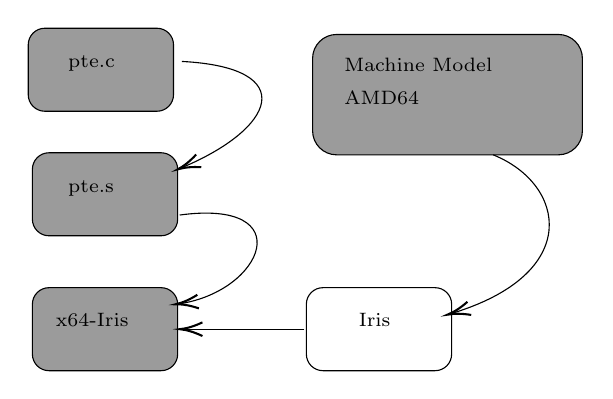
\begin{tikzpicture}[x=0.75pt,y=0.75pt,yscale=-1,xscale=1]
%uncomment if require: \path (0,201); %set diagram left start at 0, and has height of 201

%Rounded Rect [id:dp9674022449831219] 
\draw  [fill={rgb, 255:red, 155; green, 155; blue, 155 }  ,fill opacity=1 ] (49,141) .. controls (49,136.58) and (52.58,133) .. (57,133) -- (111,133) .. controls (115.42,133) and (119,136.58) .. (119,141) -- (119,165) .. controls (119,169.42) and (115.42,173) .. (111,173) -- (57,173) .. controls (52.58,173) and (49,169.42) .. (49,165) -- cycle ;
%Rounded Rect [id:dp2624123472522688] 
\draw   (181,141) .. controls (181,136.58) and (184.58,133) .. (189,133) -- (243,133) .. controls (247.42,133) and (251,136.58) .. (251,141) -- (251,165) .. controls (251,169.42) and (247.42,173) .. (243,173) -- (189,173) .. controls (184.58,173) and (181,169.42) .. (181,165) -- cycle ;
%Rounded Rect [id:dp6259709693060862] 
\draw  [fill={rgb, 255:red, 155; green, 155; blue, 155 }  ,fill opacity=1 ] (49,76) .. controls (49,71.58) and (52.58,68) .. (57,68) -- (111,68) .. controls (115.42,68) and (119,71.58) .. (119,76) -- (119,100) .. controls (119,104.42) and (115.42,108) .. (111,108) -- (57,108) .. controls (52.58,108) and (49,104.42) .. (49,100) -- cycle ;
%Rounded Rect [id:dp01887654130349059] 
\draw  [fill={rgb, 255:red, 155; green, 155; blue, 155 }  ,fill opacity=1 ] (184,22.6) .. controls (184,16.19) and (189.19,11) .. (195.6,11) -- (302.4,11) .. controls (308.81,11) and (314,16.19) .. (314,22.6) -- (314,57.4) .. controls (314,63.81) and (308.81,69) .. (302.4,69) -- (195.6,69) .. controls (189.19,69) and (184,63.81) .. (184,57.4) -- cycle ;
%Rounded Rect [id:dp43251333121558844] 
\draw  [fill={rgb, 255:red, 155; green, 155; blue, 155 }  ,fill opacity=1 ] (47,16) .. controls (47,11.58) and (50.58,8) .. (55,8) -- (109,8) .. controls (113.42,8) and (117,11.58) .. (117,16) -- (117,40) .. controls (117,44.42) and (113.42,48) .. (109,48) -- (55,48) .. controls (50.58,48) and (47,44.42) .. (47,40) -- cycle ;
%Curve Lines [id:da4125031251275959] 
\draw    (271,69) .. controls (305.83,82.93) and (314.91,126.56) .. (249.98,145.71) ;
\draw [shift={(249,146)}, rotate = 343.94] [color={rgb, 255:red, 0; green, 0; blue, 0 }  ][line width=0.75]    (10.93,-3.29) .. controls (6.95,-1.4) and (3.31,-0.3) .. (0,0) .. controls (3.31,0.3) and (6.95,1.4) .. (10.93,3.29)   ;
%Straight Lines [id:da4796300520719461] 
\draw    (180,153) -- (122,153) ;
\draw [shift={(120,153)}, rotate = 360] [color={rgb, 255:red, 0; green, 0; blue, 0 }  ][line width=0.75]    (10.93,-3.29) .. controls (6.95,-1.4) and (3.31,-0.3) .. (0,0) .. controls (3.31,0.3) and (6.95,1.4) .. (10.93,3.29)   ;
%Curve Lines [id:da6791394644184989] 
\draw    (121,24) .. controls (178.42,26.97) and (166.25,56.4) .. (120.4,75.43) ;
\draw [shift={(119,76)}, rotate = 337.99] [color={rgb, 255:red, 0; green, 0; blue, 0 }  ][line width=0.75]    (10.93,-3.29) .. controls (6.95,-1.4) and (3.31,-0.3) .. (0,0) .. controls (3.31,0.3) and (6.95,1.4) .. (10.93,3.29)   ;
%Curve Lines [id:da09850046696764791] 
\draw    (120,98) .. controls (178.12,90.12) and (160.55,134.63) .. (119.87,140.75) ;
\draw [shift={(118,141)}, rotate = 353.21] [color={rgb, 255:red, 0; green, 0; blue, 0 }  ][line width=0.75]    (10.93,-3.29) .. controls (6.95,-1.4) and (3.31,-0.3) .. (0,0) .. controls (3.31,0.3) and (6.95,1.4) .. (10.93,3.29)   ;

% Text Node
\draw (198,21) node [anchor=north west][inner sep=0.75pt]   [align=left] {\scriptsize Machine Model\\ \scriptsize AMD64};
% Text Node
\draw (205,144) node [anchor=north west][inner sep=0.75pt]   [align=left] {\scriptsize Iris};
% Text Node
\draw (59,144) node [anchor=north west][inner sep=0.75pt]   [align=left] {\scriptsize x64-Iris};
% Text Node
\draw (65,80) node [anchor=north west][inner sep=0.75pt]   [align=left] {\scriptsize pte.s};
% Text Node
\draw (65,20) node [anchor=north west][inner sep=0.75pt]   [align=left] {\scriptsize pte.c};


\end{tikzpicture}
        \caption{x64-Iris}
        \label{fig:enter-label}
    \end{figure}
    \column{0.34\textwidth}
    \begin{itemize}
        \item Dumping \textbf{.o} files
        \item Manuel treatment on \textbf{Xabs} instructions and field access
    \end{itemize}
    \end{columns}
\end{frame}
\begin{frame}{A Rough Quantification on the Current Status}\scriptsize
    \begin{table}[ht]
\centering
\caption{Line-of-Code Numbers for \textsf{pte} Verification}
\label{fig:tablepte}
\begin{tabular}[t]{lccc}
\hline
& C LoC A& Assembly LoC & Roqc Proof LoC \\
\hline
pte\_get\_next\_table&12&45& ~3200\\
pte\_walkpgdir&8&44& ~3200\\
pte\_p2v&--&1&~75\\
pte\_switch\_addrspace&--&18&~350\\
pte\_map\_page&7&28&~1750\\
pte\_initialize&4&20&~700\\
\hline
\end{tabular}
\end{table}%
\begin{table}[ht]
\centering
\vspace{-5mm}
\caption{Line-of-Code Numbers for x64-Iris Logic}
\label{fig:tablex64iris}
\begin{tabular}[t]{lc}
\hline
& Roqc LoC  \\
\hline
Soundness of Instructions Mentioned in the Presentation  &\begin{array}{l}  &  \quad \quad \quad\quad \quad\quad \quad\quad \quad 50176  \\ &(\textsf{The Complete Set of Instructions } $\ge$ 1 \textsf{ Million})\end{array}\\
VMM Related Logical Constructions &5554\\
Machine Model & 6172\\
\hline
\end{tabular}
\end{table}
\end{frame}
\section{The Current and Future Directions \& Conclusions}
\subsection{Modal Abstractions for Verification Patterns}
%begin{frame}{Resource and its Context}
 %   \begin{definition}[Resource]
 %%   \end{definition}
   % \begin{definition}[Resource Context]
   % \end{definition}
   % \begin{definition}[Nominalization]
   % \end{definition}
%\end{frame}
%------------------

%--------------
\makepart{Modal Understanding of Specification Evolution}
\begin{frame}{Protocols}
    \
\end{frame}
\begin{frame}{Specifying Protocols for Systems with \textbf{STS}es}\scriptsize
\begin{columns}[c]
\column{0.45\textwidth}
\begin{figure}
    \centering
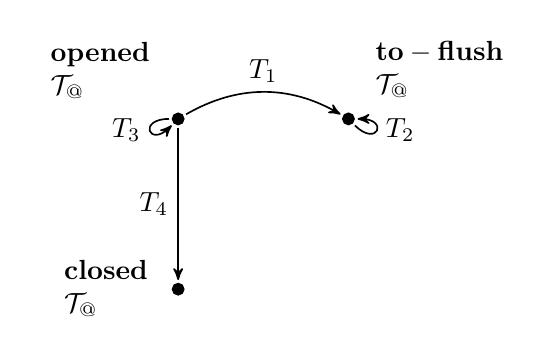
\begin{tikzpicture}[modal]
    \node[point] (to-flush) [label=135:{$\begin{array}{l}\mathbf{opened} \\ \mathcal{T}_@\end{array}$}] {};
    \node[point] (opened) [right=of to-flush, label=60:{$\begin{array}{l}\mathbf{to-flush}\\\mathcal{T}_@  
    \end{array}$}] {};
    \node[point](closed) [below=of to-flush, label=180:{$\begin{array}{l}\mathbf{closed}\\\mathcal{T}_@ 
    \end{array}$}] {};
    \path[->] (to-flush) edge[bend left] node[above]{$T_1$} (opened);
    \path[->] (opened) edge[reflexive right,out=-45,in=0,looseness=18] node[right] {$T_2$} (opened);
    \path[->] (to-flush) edge[reflexive left,out=180,in=225,looseness=18] node[left] {$T_3$} (to-flush);
     \path[->] (to-flush) edge node[left] {$T_4$} (closed);
\end{tikzpicture}
    \caption{STS for Distributed File Protocol}
    \label{fig:enter-label}
\end{figure}
\column{.45\textwidth}
\begin{figure}
    \centering
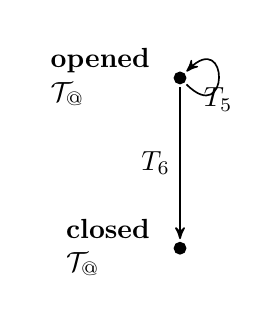
\begin{tikzpicture}[modal]
    \node[point] (opened) [label=left:{$\begin{array}{l}\mathbf{opened}\\ \mathcal{T}_@\end{array}$}] {};
     \node[point](closed) [below=of opened, label=180:{$\begin{array}{l}\mathbf{closed}\\\mathcal{T}_@ 
    \end{array}$}] {};
    \path[->] (opened) edge[reflexive right,out=-45,in=45,looseness=18] node[below] {$T_5$} (opened);
      \path[->] (opened) edge node[left] {$T_6$} (closed);
\end{tikzpicture}
    \caption{STS for Traditional File Protocol}
    \label{fig:enter-label}
    \end{figure}
\end{columns}
\begin{block}{Interacting with \textbf{STS}es}
 Modelling interactions of a client with a state machine via \emph{token exchange}
\end{block}
\end{frame}
%------------------------------------------------
\begin{frame}{Defining \textbf{STS}es}\scriptsize
\begin{definition}[\textbf{STS} Definition following CaReSL's presentation~\cite{turon13b}]
An STS $\pi$ is given by:
\begin{enumerate}
\item a set of states $\mathcal{S}$,
\item a map from a state set of tokens $\mathcal{T} : \mathcal{S} \rightarrow \mathsf{TokSet}$,
\item a transition relation $\leadsto$ on states, which is then lifted to pairs of a state and token set:
    \[(s;T)\leadsto(s';T') \triangleq s\leadsto s' \land \mathcal{T}(s)\uplus T = \mathcal{T}(s')\uplus T'\]
\item an interpretation mapping states to state assertions $\varphi :
    \mathcal{S}\rightarrow \mathsf{Prop}$.
    \end{enumerate}
\end{definition}
\end{frame}
\begin{frame}{Propositional Kripke Model}\scriptsize
     \begin{definition}[(Propositional) Kripke Model~\cite{hughes1996new}]
    A Kripke model $\mathfrak{M}$ is a triple $(W,R,V)$ where
    \begin{itemize}
        \item $W$ is a set of ``worlds''
        \item $R\subseteq W\times W$ is a relation called the \emph{accessibility} relation between worlds
        \item $V : \mathsf{PropVar} \rightarrow \mathcal{P}(W)$ gives for each propositional variable $p$ a set of worlds $V(p)$ where $p$ is considered true
    \end{itemize}
\end{definition}
\end{frame}
\begin{frame}{Bisimulations over Kripke Models}\scriptsize
\begin{definition}[(Propositional) Bisimulation of Kripke Structures: $\mathfrak{M}\sim\mathfrak{M}'$.]
    A \emph{bisimulation} between (multimodal) Kripke structures $(W,R_{i\in I},V)$ and $(W',R'_{i\in I},V')$ is a relation $E\subseteq W\times W'$ satisfying:
 \begin{itemize}
     \item If $w \; E \;w'$, then $w$ and $w'$ satisfy the same propositional variables.
     \item If $w \; E \;w'$ and $w \; R \; v$, then there exists $v'\in W'$ such that $v\;E\;v'$ and $w'\;R'\;v'$
       \item If $w \; E \;w'$ and $w'\;R'\;v'$, then there exists $v\in W$ such that $v\;R\;v'$ and $w\;R\;v$
    \end{itemize}   
\end{definition}
\end{frame}

\section{Motivation}
\subsection{Indistinguishability of Machines}
\begin{frame}{Intuition on Bisimulations over \textbf{STS}es}\scriptsize
\begin{columns}[c]
\column{0.45\textwidth}
\begin{figure}
    \centering
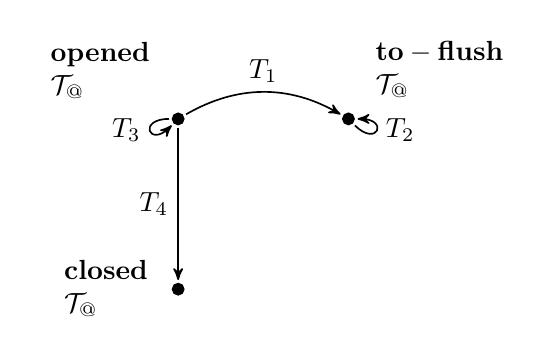
\begin{tikzpicture}[modal]
    \node[point] (to-flush) [label=135:{$\begin{array}{l}\mathbf{opened} \\ \mathcal{T}_@\end{array}$}] {};
    \node[point] (opened) [right=of to-flush, label=60:{$\begin{array}{l}\mathbf{to-flush}\\\mathcal{T}_@  
    \end{array}$}] {};
    \node[point](closed) [below=of to-flush, label=180:{$\begin{array}{l}\mathbf{closed}\\\mathcal{T}_@ 
    \end{array}$}] {};
    \path[->] (to-flush) edge[bend left] node[above]{$T_1$} (opened);
    \path[->] (opened) edge[reflexive right,out=-45,in=0,looseness=18] node[right] {$T_2$} (opened);
    \path[->] (to-flush) edge[reflexive left,out=180,in=225,looseness=18] node[left] {$T_3$} (to-flush);
     \path[->] (to-flush) edge node[left] {$T_4$} (closed);
\end{tikzpicture}
   % \caption{Caption}
    \label{fig:enter-label}
\end{figure}
\column{.45\textwidth}
\begin{figure}
    \centering
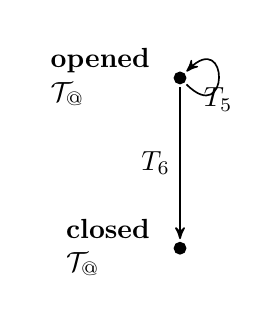
\begin{tikzpicture}[modal]
    \node[point] (opened) [label=left:{$\begin{array}{l}\mathbf{opened}\\ \mathcal{T}_@\end{array}$}] {};
     \node[point](closed) [below=of opened, label=180:{$\begin{array}{l}\mathbf{closed}\\\mathcal{T}_@  
    \end{array}$}] {};
    \path[->] (opened) edge[reflexive right,out=-45,in=45,looseness=18] node[below] {$T_5$} (opened);
      \path[->] (opened) edge node[left] {$T_6$} (closed);
\end{tikzpicture}
   % \caption{Caption}
    \label{fig:enter-label}
    \end{figure}
\end{columns}
\begin{itemize}
    \item More than just relating \textbf{STS}es in representation invariants per state.
    \item Bisimilar states can have different representation invariants.
    \end{itemize}
    \begin{alertblock}{Proof Indistinguishability}
        Knowing the proof of a client against the right (target STS conventionally $\pi'$)  \emph{enables} deducing the proof against the bisimilar on the left (source STS conventionally $\pi$).
    \end{alertblock}   
\end{frame}
\begin{frame}{A Quick Tour on \textbf{STS} Assertions}\scriptsize
\begin{itemize}
    \item Invariants $\fbox{$\varphi$}^{\gamma}_{\pi}$,  client capability $\ownGhost{\gamma}{s;\mathsf{T}}$
\end{itemize}
\begin{figure}
\centering
\scriptsize
\[
\begin{array}{l}
 \inferrule[STSAlloc]{ }{
    \varphi(s) \vs \exists \gamma \ldotp \fbox{$\varphi$}^{\gamma}_{\pi} \ast \ownGhost{\gamma}{s;\mathsf{AllTokens}\setminus\mathcal{T}(s)}
}\\
 \inferrule[STSOpen]{ }{
 \fbox{$\varphi$}^{\gamma}_{\pi} \ast \ownGhost{\gamma}{s;\mathsf{T}} \vs (\exists \; s' \ldotp \ulcorner  (\mathsf{s}0, \mathsf{T}) \overset{\mathsf{rely}^{*}}{\sqsubseteq}_{\pi} (\mathsf{s}',\mathsf{T}) \urcorner \ast \varphi(s) \ast \forall \mathsf{sl}', \;\mathsf{T}' \ldotp
      \ulcorner (\mathsf{s'}, \mathsf{T}) \overset{\mathsf{guar.}^{*}}{\sqsubseteq}_{\pi} (\mathsf{sl}', \mathsf{T}') \urcorner \ast \varphi(\mathsf{sl}') \vs \ownGhost{\gamma}{\mathsf{sl};\mathsf{T}'} )
 } \\
 \inferrule[UpdIsl]{
        \alpha~\textrm{physically atomic}\\
        \forall s_0 \;\ldotp  \;((s;\mathsf{T})\;\overset{\mathsf{rely}^{*}}{\sqsubseteq}_\pi\;( s_0;\mathsf{T}))\; \vdash
        \triple{ \varphi(s_0)\ast P }{\alpha}{ \exists s' \;, \;\mathsf{T}'\;\ldotp \; (s_0;\mathsf{T})\; \overset{\mathsf{guar}^{*}}{\sqsubseteq}_\pi \;(s';\mathsf{T}') \ast 
        \varphi(s')\ast Q}
    }{
      \fbox{$\varphi$}^{\gamma}_{\pi} \vdash
      \triple{ \ownGhost{\gamma}{s;\mathsf{T}} \ast P }
            {\alpha}
        { \exists \; s', \mathsf{T}' \ldotp \ownGhost{\gamma}{s';\mathsf{T}'} \ast Q }
    }
 \end{array}
\]
\vspace{-1em}
\caption{Iris STS Library ~\cite{Jung2015Iris} simplified with \textsf{later modality} and \textsf{invariant masks} omitted}
  \label{fig:stslib}
\end{figure}
\end{frame}
\section{Logic}
\subsection{Iris \textbf{STS} Library}
\begin{frame}{Decomposing Bisimilarity in \textbf{STS}es}\scriptsize
\begin{columns}
\column{0.4\textwidth}
The bisimulation ($\mathcal{M}(\pi,\pi',\varphi,\varphi',s,\mathsf{T},\mathsf{U})$) between two state machines, $\pi$ and $\pi'$ is composed of 
\begin{itemize}
\item The source STS -- $\pi$
\item The target STS -- $\pi'$
\item The source STS's state interpretation function -- $\varphi$
\item The target STS's state interpretation function -- $\varphi'$
    \item Token Embedding -- $\epsilon_{\mathcal{S}} : \;\; \mathcal{S}(\pi) \mapsto \mathcal{S}(\pi')$
    \item State Embedding -- $\epsilon_{\mathcal{T}} :\;\;  \mathcal{T}(\pi) \mapsto \mathcal{T}(\pi')$
    \item The Law of Rely 
    \item The Law of Guarantee
    \item The Law of Tolerance
    \item The state of source STS from which bisimulation is considered against any client interference with the token set $T$
\end{itemize}
\column{0.59\textwidth}
\begin{alertblock}{Proof Translation}
     Obtain a proof rule utilizing the bisimulation to translate proofs between bisimilar state machines!
\end{alertblock}
\end{columns}
\end{frame}
\subsection{Understanding Bisimulations}

\begin{frame}{We Need This} \scriptsize
\[
\inferrule[Bisim]{
	\pi\sim\pi'\quad\quad 
	q\; \epsilon_{\mathcal{S}} \;s \quad\quad q' \; \epsilon_{\mathcal{S}} \;s' \\
	\triple{\ownGhost{\gamma}{s;\epsilon_{\overline{\mathcal{T}}}(\mathcal{T})}_{\pi'} \ast P}{C}{\ownGhost{\gamma}{s';\mathsf{T}'}_{\pi'} \ast Q}
}{
	\fbox{$\varphi$}^{\gamma}_{\pi} \vdash
    \triple{\ownGhost{\gamma}{q;\mathsf{T}}_{\pi}\ast P}{C}{\ownGhost{\gamma}{q';\mathsf{T}'}_{\pi} \ast Q}
}
\]
\end{frame}
\begin{frame}{We Use This}\scriptsize
\[
\inferrule[UpdIsl]{
        \alpha~\textrm{physically atomic}\\
        \forall s_0 \;\ldotp  \;((s;\mathsf{T})\;\overset{\mathsf{rely}^{*}}{\sqsubseteq}_\pi\;( s_0;\mathsf{T}))\; \vdash
        \triple{ \varphi(s_0)\ast P }{\alpha}{ \exists s' \;, \;\mathsf{T}'\;\ldotp \; (s_0;\mathsf{T})\; \overset{\mathsf{guar}^{*}}{\sqsubseteq}_\pi \;(s';\mathsf{T}') \ast 
        \varphi(s')\ast Q}
    }{
      \fbox{$\varphi$}^{\gamma}_{\pi} \vdash
      \triple{ \ownGhost{\gamma}{s;\mathsf{T}} \ast P }
            {\alpha}
        { \exists \; s', \mathsf{T}' \ldotp \ownGhost{\gamma}{s';\mathsf{T}'} \ast Q }
    }
\]
\[
\inferrule[Bisim]{
	\pi\sim\pi'\quad\quad 
	q\; \epsilon_{\mathcal{S}} \;s \quad\quad q' \; \epsilon_{\mathcal{S}} \;s' \\
	\triple{\ownGhost{\gamma}{s;\epsilon_{\overline{\mathcal{T}}}(\mathcal{T})}_{\pi'} \ast P}{C}{\ownGhost{\gamma}{s';\mathsf{T}'}_{\pi'} \ast Q}
}{
	\fbox{$\varphi$}^{\gamma}_{\pi} \vdash
    \triple{\ownGhost{\gamma}{q;\mathsf{T}}_{\pi}\ast P}{C}{\ownGhost{\gamma}{q';\mathsf{T}'}_{\pi} \ast Q}
}
\]
\end{frame}
\begin{frame}{Invariants of File Protocols} \scriptsize
\begin{definition}[File Protocol Invariants]    
    \[
\varphi_{\mathsf{distributedfile}} \;(\;\ell\;, \;\mathsf{R}\;)( \;s \; )\;\triangleq \;
\left\{
\begin{array}{cc}
\mathsf{match}\; \mathsf{s} \; \mathsf{with}\\
  \mathsf{to-flush} \Rightarrow  &  \mathsf{R} \ast \exists \; \mathsf{fs} \ldotp \mathsf{isValidDirty}(\mathsf{fs}) \ast \\ & \quad\quad\quad\quad \ell \mapsto (\mathsf{fs}.id,\mathsf{fs}.\mathsf{status}=\mathsf{dirty})  \\
   \mathsf{opened} \Rightarrow  &  \mathsf{R} \ast \exists \; \mathsf{fs} \ldotp \mathsf{isValid}(\mathsf{fs}) \ast \\ & \quad\quad\quad\quad \ell \mapsto (\mathsf{fs}.id,\mathsf{fs}.\mathsf{status}=\mathsf{clean}) \\
   \mathsf{closed} \Rightarrow  & \exists \; \mathsf{fs} \ldotp \mathsf{isValidClosed}(\mathsf{fs}) \ast \\ & \quad\quad\quad\quad \ell \mapsto (\mathsf{fs}.id,\mathsf{fs}.\mathsf{status}=\textsf{closed}) 
\end{array}
\right\}
\]
\[
\varphi_{\mathsf{file}} \;(\;\ell \;\mathsf{R}\;)( \;s \;)\; \triangleq \;
\left\{
\begin{array}{cc}
\mathsf{match}\; \mathsf{s} \; \mathsf{with}\\
   \mathsf{opened} \Rightarrow  &  \mathsf{R} \ast \exists \; \mathsf{fs} \ldotp \mathsf{isValid}(\mathsf{fs}) \ast \ell \mapsto (\mathsf{fs}.id,\mathsf{fs}.\mathsf{status}=\mathsf{clean} \lor \mathsf{dirty}) \\
   \mathsf{closed} \Rightarrow  & \exists \; \mathsf{fs} \ldotp \mathsf{isValidClosed}(\mathsf{fs}) \ast \ell \mapsto (\mathsf{fs}.id,\mathsf{fs}.\mathsf{status}=\mathsf{closed}) 
\end{array}
\right\}
\]
\end{definition}
\end{frame}
\begin{frame}{Keeping Promises}
    \[
\inferrule[Transfer File Write]{
	\pi\sim\pi'\quad\quad 
	\mathsf{opened}\; \epsilon_{\mathcal{S}} \;s \quad\quad q' \; \epsilon_{\mathcal{S}} \;s' \\
	\triple{\ownGhost{\gamma}{s;\epsilon_{\overline{\mathcal{T}}}(\mathcal{T})}_{\pi'} \ast P}{\mathsf{write}\; \ell \; \mathsf{new\_val}}{\ownGhost{\gamma}{s';\mathsf{T}'}_{\pi'} \ast Q}
}{
	\fbox{$\varphi_{\mathsf{distributedfile}}$}^{\gamma}_{\pi} \vdash
    \triple{\ownGhost{\gamma}{\mathsf{opened};\mathsf{T}}_{\pi}\ast P}{\mathsf{write}\; \ell \; \mathsf{new\_val}}{\ownGhost{\gamma}{q';\mathsf{T}'}_{\mathsf{\pi}} \ast Q}
}
\]
\end{frame}
\begin{frame}{The Law of Rely}\scriptsize
 \begin{theorem}[The Law of Rely]\scriptsize
            \[
            \begin{array}{l}\forall s' .   (s;T) \overset{\mathsf{rely}^{*}}{\sqsubseteq}_{\pi}  (s';T) \leftrightarrow \\
           \quad\quad  (\forall_{s_1,s_1',T_1} \ldotp \epsilon_{\mathcal{S}}(s ,s_1) \rightarrow \epsilon_{\mathcal{S}}(s',s'_1) \rightarrow \epsilon_{\overline{\mathcal{T}}}(T,T_1) \rightarrow ( s_1; T_1) \overset{\mathsf{rely}^{*}}{\sqsubseteq}_{\pi'} (s'_1; T_1)
            \end{array}
           \]
     \end{theorem}
     \begin{itemize}
         \item We do not drop any client interference with capabilities $T$
         \item Indetification of the states that are tolerant to the client interference from which the STS can take steps (Guarantee)
         \item Bookkeeping of the client interference needed!  
         \item Identifying the valid \emph{pre} state
     \end{itemize}
\end{frame}
\begin{frame}{The Law of Guarantee}\scriptsize
    \begin{theorem}[Guarantee Bisim without Invariants] 
\[
\begin{array}{l}
\forall_{q',q, T'} \ldotp 
    \epsilon_{\overline{\mathcal{T}}} ( T) \equiv T' \rightarrow \epsilon_{\mathcal{S}}(s,q)
\rightarrow   (q;T')\overset{\mathsf{rely}^{*}}{\sqsubseteq}_{\pi'}(q';T') \rightarrow  \\
\quad\quad\quad\quad \forall_{q'',T''}\ldotp (q';T')\overset{\mathsf{guar.}}{\sqsubseteq}_{\pi'}(q'';T'') \rightarrow  \\
\quad\quad\quad\quad\quad\quad \exists_{s',s'',T'_0,T''_0} \ldotp (s';T'_0) \overset{\mathsf{guar.}}{\sqsubseteq}_{\pi} (s'';T''_0) \land \\ \quad\quad\quad\quad\quad\quad\quad\quad \epsilon_{\mathcal{S}}(s')=q' \land \epsilon_{\mathcal{S}}(s'') = q'' \land \epsilon_{\overline{\mathcal{T}}}(T'_0) \equiv T' \land \epsilon_{\overline{\mathcal{T}}}(T''_0) \equiv T''
 \end{array}
\]
\end{theorem}
\begin{itemize}
    \item \emph{Under the embedded client interference}, the steps taken by the target STS must be countered by a one in the source STS
    \item From target STS to source STS
    \item Identifying the valid \emph{post} state 
\end{itemize}
\end{frame}
\begin{frame}{Soundness}
\begin{theorem}[Soundness]
    The updated state from \textsc{UpdIsl} is preserved by the bisimulation.
\end{theorem}
\end{frame}


\section{The Current and Future Directions \& Conclusions}
\begin{frame}{Ongoing Work}
    \begin{itemize}
        \item Bisimulation over Restricted Submodels
        \begin{itemize}
            \item We need to  strengthen the bisimulation 
            \item What is this strength? 
            \begin{itemize}
                \item Guarantee steps taken at the target machine with $T\setminus U$ has to be indistinguishable (entail) the ones taken with $T$
                \item \textbf{The Law of Abduction}: Knowing more about $U$ and capabilities dropped with the absence of it.

            \end{itemize}
            
        \end{itemize}
        \item Extending Rules for the Complete Iris \textsc{HeapLang}
                        \item  An abstract framework with relational \emph{embeddings} is finished and written. 
                        \begin{itemize}
                            \item Subjectively more promising!
                            \item We need to justify concretely via an example, that is, an example exposes incapability of current non-relational embeddings of states and tokens \end{itemize}
                        \end{itemize}
\end{frame}
\begin{frame}{The Future Directions}
    \begin{itemize}
        \item Exploit obvious application fields, e.g., device drivers
        \item Only Iris pluggable?
    \end{itemize}
\end{frame}
\makepart{Semantic Type Assertion for Deferred Memory-Reclamation Schemes \\ ESOP'19}
\section{Deferred Memory Reclamation}
\begin{frame}{What is Deferred Memory Reclamation?}
    \begin{itemize}
        \item Both \emph{reader} and \emph{writer} threads accessing to a memory location \emph{simultaneously}
        \item The write \emph{waits} the readers that are already on the same memory location --- i.e., \emph{Grace Period}
        \item After the grace period end, the grace period ends, i.e, the readers leave the memory location, it is safe to \emph{reclaim} the memory location
        \item Different schemes: Hazard Pointers, Read-Copy-Update \cite{}
    \end{itemize}
\end{frame}

\begin{frame}{RCU Semantics}\scriptsize
\begin{figure}[H]
 \centering
 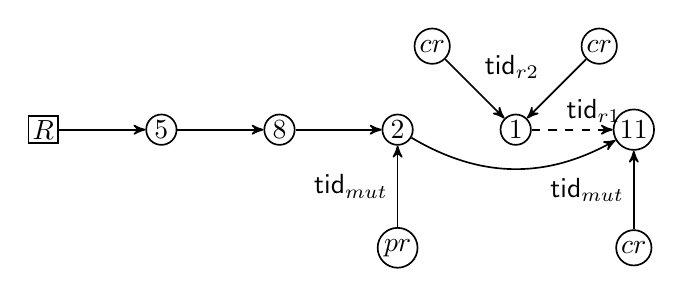
\begin{tikzpicture}[>=stealth',node distance=1.5cm,semithick,auto]
 \tikzstyle{hollow node}=[circle,draw,inner sep=1]
 \tikzstyle{sub node}=[triangle,draw,inner sep=1]
 \tikzstyle{solid node}=[rectangle,draw,inner sep=1.5]

 \tikzset{
	red node/.style={rectangle,draw=black,fill=red,inner sep=1.5},
 	blue node/.style={rectangle,draw=black,inner sep=1.5},
 	reader node/.style={circle,draw=black,inner sep=1},
 	writer node/.style={circle,draw=black,inner sep=1}
 }

       \node[solid node] (R) {$R$};
       \node[hollow node] (5) [right of=R] {$5$};
       \node[hollow node] (8) [right of=5] {$8$};
       \node[hollow node] (2) [right of=8] {$2$};
       \node[hollow node] (1) [right of=2] {$1$};
       \node[hollow node] (11) [right of=1] {$11$};
       %\node[hollow node] (4) [right of=11] {$4$};
       \node[reader node] (r1) [above right of= 1]  {$cr$};
       \node[reader node] (r2)  [above left of= 1] {$cr$};
       \node[writer node] (wp) [below of=2] {$pr$};
       \node[writer node] (wc) [below of=11]{$cr$};

     \path[->]  (R) edge node {} (5);
     \path[->]  (5) edge node {} (8);
     \path[->]  (8) edge node {} (2);
    % \path[->]  (11) edge node {} (4);
     \path[->] (2) edge [bend right] node {} (11);
     \path[dashed,->]  (1) edge node {} (11);

     \path[->]  (r1) edge node {$\textsf{tid}_{r1}$} (1);
     \path[->]  (r2) edge node {$\textsf{tid}_{r2}$} (1);
     \path[->]  (wp) edge node  {$\textsf{tid}_{mut}$}  (2);
     \path[->]  (wc) edge  node  {$\textsf{tid}_{mut}$}   (11);
 ;
 \end{tikzpicture}
 \caption{$\textsf{tid}_{mut}$ unlinks the node with value 1.}
 \label{fig:unlinkedlist}
 \end{figure}
% After \emph{mutation} in heap, -(remove:16)-, Writer thread calls \textsf{SyncStart}-(\emph{remove:14})-to start \emph{grace-period}. Now, $\textsf{tid}_{r1}$ and $\textsf{tid}_{r1}$ become \emph{bounding-threads} which $t_{mut}$ needs to wait which is shown in \ref{fig:unlinkedlist}.
 \begin{figure}[H]
 \centering
 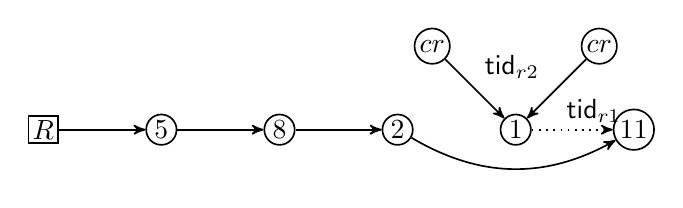
\begin{tikzpicture}[>=stealth',node distance=1.5cm,semithick,auto]
 \tikzstyle{hollow node}=[circle,draw,inner sep=1]
 \tikzstyle{sub node}=[triangle,draw,inner sep=1]
 \tikzstyle{solid node}=[rectangle,draw,inner sep=1.5]

 \tikzset{
 	red node/.style={rectangle,draw=black,fill=red,inner sep=1.5},
 	blue node/.style={rectangle,draw=black,inner sep=1.5},
 	reader node/.style={circle,draw=black,inner sep=1},
 	writer node/.style={circle,draw=black,inner sep=1}
 }

       \node[solid node] (R) {$R$};
       \node[hollow node] (5) [right of=R] {$5$};
       \node[hollow node] (8) [right of=5] {$8$};
       \node[hollow node] (2) [right of=8] {$2$};
       \node[hollow node] (1) [right of=2] {$1$};
       \node[hollow node] (11) [right of=1] {$11$};
     %  \node[hollow node] (4) [right of=11] {$4$};
       \node[reader node] (r1) [above right of= 1]  {$cr$};
       \node[reader node] (r2)  [above left of= 1] {$cr$};

     \path[->]  (R) edge node {} (5);
     \path[->]  (5) edge node {} (8);
     \path[->]  (8) edge node {} (2);
    % \path[->]  (11) edge node {} (4);
     \path[->] (2) edge [bend right] node {} (11);
     \path[dotted,->]  (1) edge node {} (11);

     \path[->]  (r1) edge node {$\textsf{tid}_{r1}$} (1);
     \path[->]  (r2) edge node {$\textsf{tid}_{r2}$} (1);

 ;
 \end{tikzpicture}
 \qquad
 \qquad
 \tikzset{
     font=\sffamily,
    BLOCK/.style={
         draw,
        align=center,
         text height=0.4cm,
         draw=red!50,
         fill=red!20,
         rectangle split,
         rectangle split horizontal,
         rectangle split parts=#1,
     }
 }
 \begin{tikzpicture}
     \node (h1) {to-free list};
     \node[BLOCK=3, below=0 of h1]{
       \nodepart{one}...\nodepart{two}( F[ s(1,$\textsf{tid}_{mut}$) $\rightharpoonup$ {$\textsf{tid}_{r1}$, $\textsf{tid}_{r2}$} ]
         \nodepart{three}...};
 \end{tikzpicture}

 \caption{Bounding threads, $\textsf{tid}_{r1}$ $\textsf{tid}_{r1}$. }
 \label{fig:unlinkedlistnomut}
 \end{figure}
% Grace period lasts until \textsf{SyncStop} returns-(\emph{remove:15})-. \textsf{SyncStop} blocks the execution of the writer thread until $\textsf{tid}_{r1}$ and $\textsf{tid}_{r2}$ exit \textsf{Read Block} as shown in figure ~\ref{fig:unlinkedlistnomut}. We use mapping, $F$, to from mutated memory locations to reader thread identifiers active when the mutation occurs.  
\end{frame}
\begin{frame}{RCU Semantics}\scriptsize
 \begin{figure}[H]
 \centering
 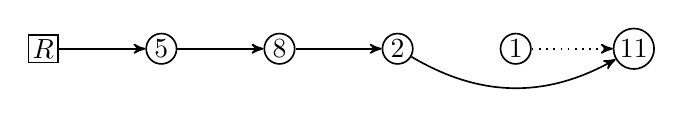
\begin{tikzpicture}[>=stealth',node distance=1.5cm,semithick,auto]
 \tikzstyle{hollow node}=[circle,draw,inner sep=1]
 \tikzstyle{sub node}=[triangle,draw,inner sep=1]
 \tikzstyle{solid node}=[rectangle,draw,inner sep=1.5]

 \tikzset{
 	red node/.style={rectangle,draw=black,fill=red,inner sep=1.5},
 	blue node/.style={rectangle,draw=black,inner sep=1.5},
 	reader node/.style={circle,draw=black,inner sep=1},
 	writer node/.style={circle,draw=green,inner sep=1}
 }

       \node[solid node] (R) {$R$};
       \node[hollow node] (5) [right of=R] {$5$};
       \node[hollow node] (8) [right of=5] {$8$};
       \node[hollow node] (2) [right of=8] {$2$};
       \node[hollow node] (1) [right of=2] {$1$};
       \node[hollow node] (11) [right of=1] {$11$};
       %\node[hollow node] (4) [right of=11] {$4$};

     \path[->]  (R) edge node {} (5);
     \path[->]  (5) edge node {} (8);
     \path[->]  (8) edge node {} (2);
     %\path[->]  (11) edge node {} (4);
     \path[->] (2) edge [bend right] node {} (11);
     \path[dotted,->]  (1) edge node {} (11);


 ;
 \end{tikzpicture}
 \qquad
 \qquad
 \tikzset{
     font=\sffamily,
     BLOCK/.style={
         draw,
         align=center,
         text height=0.4cm,
         draw=red!50,
         fill=red!20,
         rectangle split,
         rectangle split horizontal,
         rectangle split parts=#1,
     }
 }
 \begin{tikzpicture}
     \node (h1) {to-free list};
     \node[BLOCK=3, below=0 of h1]{
       \nodepart{one}...\nodepart{two} F[s(1,\textsf{tid}) $\rightharpoonup$ $\emptyset$ )
         \nodepart{three}...};
 \end{tikzpicture}
 \caption{Bounding threads, $\textsf{tid}_{r1}$ and $\textsf{tid}_{r2}$ exit \textsf{ReadBlock}. }
 \label{fig:prereclaim}
 \end{figure}
% In figure \ref{fig:prereclaim}, $\textsf{tid}_{r1}$ and $\textsf{tid}_{r2}$ exit \textsf{ReadBlock} so that \textsf{Free} can be called to reclaim the memory. Once \textsf{Free} returns, the memory location is reclaimed as shown in figure \ref{fig:reclaimed}. 
 \begin{figure}[H]
 \centering
 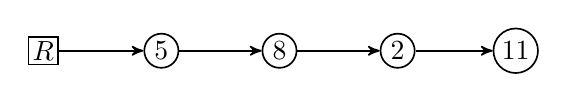
\begin{tikzpicture}[>=stealth',node distance=1.5cm,semithick,auto]
 \tikzstyle{hollow node}=[circle,draw,inner sep=1.5]
 \tikzstyle{sub node}=[triangle,draw,inner sep=1]
 \tikzstyle{solid node}=[rectangle,draw,inner sep=1.5]

 \tikzset{
 	red node/.style={rectangle,draw=red,fill=red,inner sep=1.5},
 	blue node/.style={rectangle,draw=black,inner sep=1.5},
 	reader node/.style={circle,draw=black,inner sep=1},
 	writer node/.style={circle,draw=green,inner sep=1}
 }

       \node[solid node] (R) {$R$};
       \node[hollow node] (5) [right of=R] {$5$};
       \node[hollow node] (8) [right of=5] {$8$};
       \node[hollow node] (2) [right of=8] {$2$};
       \node[hollow node] (11) [right of=2] {$11$};
 %      \node[hollow node] (4) [right of=11] {$4$};

     \path[->]  (R) edge node {} (5);
     \path[->]  (5) edge node {} (8);
     \path[->]  (8) edge node {} (2);
  %   \path[->]  (11) edge node {} (4);
     \path[->] (2) edge node {} (11);
 ;
 \end{tikzpicture}
 \caption{ Reclaimed the node 1}
 \label{fig:reclaimed}
 \end{figure}
% Another interesting mutation on the heap of the \textsf{RCU} bag is \emph{fresh-node-linking} case which shows up in \emph{add} method. The mutator thread, $t_{mut}$, allocates a fresh node, $n$, in the heap-(\emph{add:8})-and links the newly allocated node the list-(\emph{add:17}).
% We see in figure \ref{fig:freshlist} that the linked list is in a state where there exists two entry points, $R$ and $n$, to it. This seems to be a violation of well-formedness of the linked list at first. However, the dash-dot type--\emph{fresh}--of link in between fresh node and \textsf{RCU} data structure still preserves well-formedness as straight arrows are the only types--\emph{iterator}-- that one can use to access to the \textsf{RCU} data structure. The dash-dot type turns into a stright arrow in figure \ref{fig:freshlistlinked} once the freshly allocated node, $n$, is linked to the \textsf{RCU} list.
\end{frame}
\begin{frame}{Type Assertions for RCU}
\begin{figure*}[t!]
\begin{tabular}{p{0.47\textwidth}p{0.47\textwidth}}
\begin{lstlisting}[basicstyle=\scriptsize\ttfamily]
struct BagNode{
  int data;
  BagNode<rcuItr> Next;
}
BagNode<rcuRoot> head;
void add(int toAdd){
WriteBegin;
BagNode nw = new;
$\assert{nw\mathsf{:rcuFresh}  \{\}}$
nw.data = toAdd;
$\assert{head\mathsf{:rcuRoot},par\mathsf{:undef}, cur\mathsf{:undef}}$
BagNode<rcuItr> par,cur = head;
$\assert{head\mathsf{:rcuRoot},par\mathsf{:rcuItr} \epsilon  \{\}}$
$\assert{cur\mathsf{:rcuItr} \epsilon  \{\}}$
cur = par.Next;
$\assert{cur\mathsf{:rcuItr} Next \{\}}$
$\assert{par\mathsf{:rcuItr} \epsilon \{Next\mapsto cur\}}$
while(cur.Next != null){
  $\assert{cur\mathsf{:rcuItr} (Next)^{k}.Next \{\}}$
  $\assert{par\mathsf{:rcuItr}  (Next)^{k} \{Next \mapsto cur\}}$
  par = cur;
  cur = par.Next;
  $\assert{cur\mathsf{:rcuItr} (Next)^{k}.Next.Next \{\}}$
  $\assert{par\mathsf{:rcuItr}(Next)^{k}.Next \{Next \mapsto cur\}}$
}
$\assert{nw\mathsf{:rcuFresh}  \{\}}$
$\assert{cur\mathsf{:rcuItr} (Next)^{k}.Next \{Next\mapsto null\}}$
$\assert{par\mathsf{:rcuItr}  (Next)^{k} \{Next \mapsto cur\}}$
nw.Next= null;
$\assert{nw\mathsf{:rcuFresh}  \{Next\mapsto null\}}$
$\assert{cur\mathsf{:rcuItr} (Next)^{k}.Next \{Next \mapsto null\} }$
cur.Next=nw;
$\assert{nw\mathsf{:rcuItr}  (Next)^{k}.Next.Next  \{Next\mapsto null\}}$
$\assert{cur\mathsf{:rcuItr} (Next)^{k}.Next \{Next \mapsto nw\} }$
WriteEnd;
}
\end{lstlisting}&
\begin{lstlisting}[basicstyle=\scriptsize\ttfamily]
void remove(int toDel){
WriteBegin;
$\assert{head\mathsf{:rcuRoot},par:\mathsf{undef}, cur\mathsf{:undef}}$
BagNode<rcuItr> par,cur = head;
$\assert{head\mathsf{:rcuRoot},par\mathsf{:rcuItr}\epsilon  \{\},cur\mathsf{:rcuItr} \epsilon  \{\}}$
cur = par.Next;
$\assert{cur\mathsf{:rcuItr} Next \{\}}$
$\assert{par\mathsf{:rcuItr} \epsilon \{Next\mapsto cur\}}$
while(cur.Next != null&&cur.data != toDel)
{
  $\assert{cur\mathsf{:rcuItr} (Next)^{k}.Next \{\}}$
  $\assert{par\mathsf{:rcuItr}  (Next)^{k} \{Next \mapsto cur\}}$
  par = cur;
  cur = par.Next;
  $\assert{cur\mathsf{:rcuItr} (Next)^{k}.Next.Next \{\}}$
  $\assert{par\mathsf{:rcuItr}  (Next)^{k}.Next \{Next \mapsto cur\}}$
}
$\assert{nw\mathsf{:rcuFresh} \{\}}$
$\assert{par\mathsf{:rcuItr}  (Next)^{k} \{Next \mapsto cur\}}$
$\assert{cur\mathsf{:rcuItr} (Next)^{k}.Next \{\}}$
BagNode<rcuItr> curl = cur.Next;
$\assert{cur\mathsf{:rcuItr} (Next)^{k}.Next \{Next \mapsto curl\}}$
$\assert{curl\mathsf{:rcuItr} (Next)^{k}.Next.Next \{\}}$
par.Next = curl;
$\assert{par\mathsf{:rcuItr}  (Next)^{k} \{Next \mapsto curl\}}$
$\assert{cur\mathsf{:unlinked}}$
$\assert{cur\mathsf{:rcuItr} (Next)^{k}.Next \{\}}$
SyncStart;
SyncStop;
$\assert{cur\mathsf{:freeable}}$
Free(cur);
$\assert{cur\mathsf{:undef}}$
WriteEnd;
}
\end{lstlisting}
%\end{minipage}
%\end{tabular*}
\end{tabular}
\vspace{-2em}
\caption{RCU client: singly linked list based bag implementation.}
\label{fig:rculist}
\end{figure*}
\end{frame}

\begin{frame}{A Taste of Soundness on Type System for RCU}
\begin{itemize}
    \item Soundness on top of Views Framework (Dinsdale-Young et.al. ~\cite{})
    \begin{itemize}
        \item Logical state with its observation-map , free-list etc. 
        \item Denotation of types encoding the post-environment of any type accurately
        \[\llbracket \Gamma,\, x:\textsf{rcuItr} \, \rho \, \mathcal{N}[y:\textsf{rcuItr}]  \rrbracket_{M,tid}\]
    \end{itemize}
    \item Global Invariants
    \begin{itemize}
        \item Unlinked Reachability:
        \item Delayed Ownership Transfer and Reader in Freelist:
    \end{itemize}
    \item Discharging these invariants once as a part of soundness
    \begin{itemize}
        \item No need to prove them for each different client
    \end{itemize}
\end{itemize}
\end{frame}
\begin{frame}{Remarks}
    \begin{itemize}
        \item Simpler that full-blown program logics: Tassarotti et al. ~\cite{}, Fu et.al. ~\cite{}, Gotsman et.al. ~\cite{}
        \item The first general operational model for RCU-based memory management
        \item Based on our suitable abstractions for RCU in the operational semantics 
        \begin{itemize}
            \item Decoupling the memory-safety proofs from the underlying reclamation model
            \item Similar is done for correctness by Meyer and Wolff ~\cite{}
        \end{itemize}
        \item Applicability/Usability
        \begin{itemize}
            \item The first safety proof RCU client Citrus Binary Search Tree (Arbel ~\cite{})
            \item Linked-list based bag implementation (McKenney Technical Report 2015)
        \end{itemize}
        \item More type rules in the paper
        \begin{itemize}
            \item Refinement rules for control flows 
            \item A simple type system for readers
            \item Entering and exiting read/write-side critical sections
        \end{itemize}
    \end{itemize}
\end{frame}
\begin{frame}{Future Directions}
    \begin{itemize}
        \item Deploying it as Clang front-end
        \begin{itemize}
            \item Abstract operational semantics can handle “classical RCU”
            \item But optimized “batch lists” in Linux kernel? Refinement with our abstract model?
        \end{itemize}
        \item Rust ownership
        \begin{itemize}
            \item When published Rust's ownership was not able to handle RCU-like programming pattern
            \item Now there is a set of RCU types
        \end{itemize}  
        \item Go adopted similar pattern in the existence of garbage-collector
        \begin{itemize}
            \item Captured by our operational semantics 
            \item Async-free + Free list
        \end{itemize}
        \item Beyond memory-safety? Tolerance to \emph{stale data}
    \end{itemize}
\end{frame}
%------------------------------------------------
%\begin{frame}{References}\scriptsize
    \scriptsize
    \bibliography{reference.bib}
    \bibliographystyle{ACM-Reference-Format}

%----------------------------------------------------------------------------------------

\end{document}


